\chapter{Relational Database Service (RDS)}\label{ch:relational-database-service}

Amazon RDS is a service which allows developers to create fully-featured and highly-available SQL databases that can be
automatically replicated to additional availability zones.
To create an Amazon RDS instance, a suitable identifier for the database is required before created, as well as a
selection of the resource limits for the virtual server.
The database requires a username and passphrase, although for additional security there is the option to automatically
generate a passphrase.
Afterwards, the type of SQL database required (such as MySQL, PostgreSQL, MariaDB or others) will be selected and then
the database should begin provisioning.

\section{Creation of RDS}\label{sec:creation-of-rds}
Password authentication was used for accessing the RDS instance as the accounts used to develop this deployment were
denied permissions from the root user to create IAM roles within this environment.
In the future, it would be recommended to select one of the other options to improve security, however this was not
possible for the project.

\begin{figure}[!htbp]
    \centering
    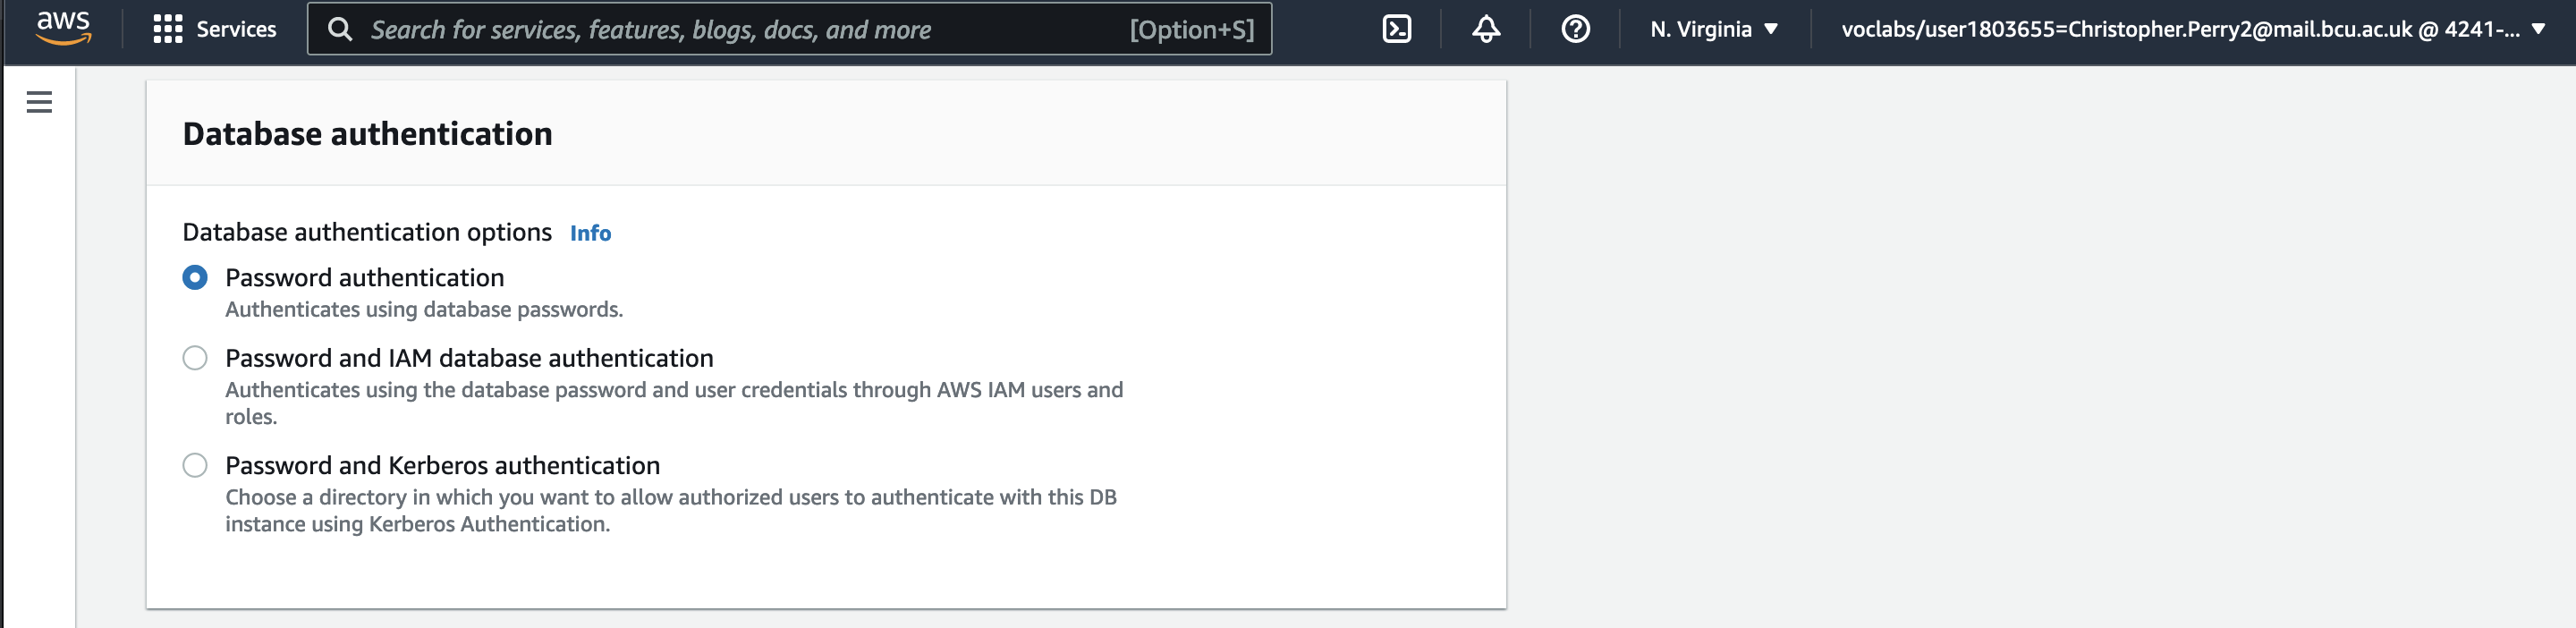
\includegraphics[width=\textwidth]{resources/rds/rds-authentication}
    \caption{Selection of RDS authentication options.}
    \label{fig:rds-auth}
\end{figure}

\clearpage
Additionally, an instance with multiple availability zones was selected to ensure that the database was highly
available and that the web app would still be able to access information from the database if one availability
zone becomes unavailable.

\begin{figure}[!htbp]
    \centering
    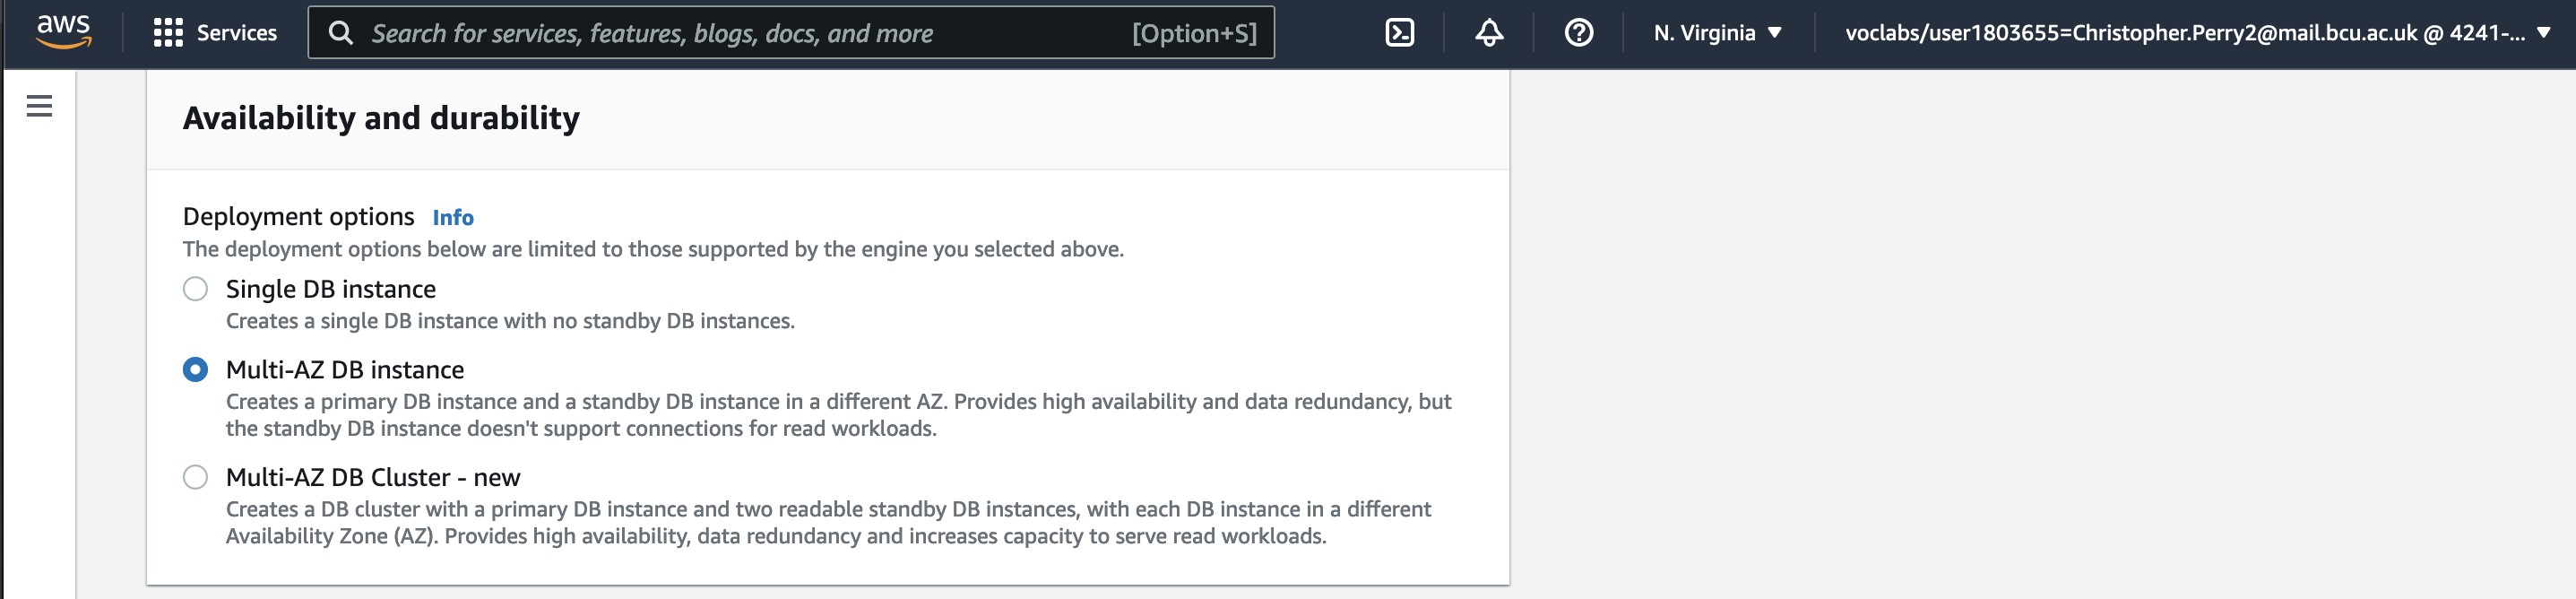
\includegraphics[width=\textwidth]{resources/rds/rds-availability-durability}
    \caption{Selection RDS multiple availability zones.}
    \label{fig:rds-avail}
\end{figure}

While configuring the RDs instance, it was also required to select a VPC to use.
The VPC created earlier in this deployment was used.
Public access to the database was turned off to further increase security.

\begin{figure}[!htbp]
    \centering
    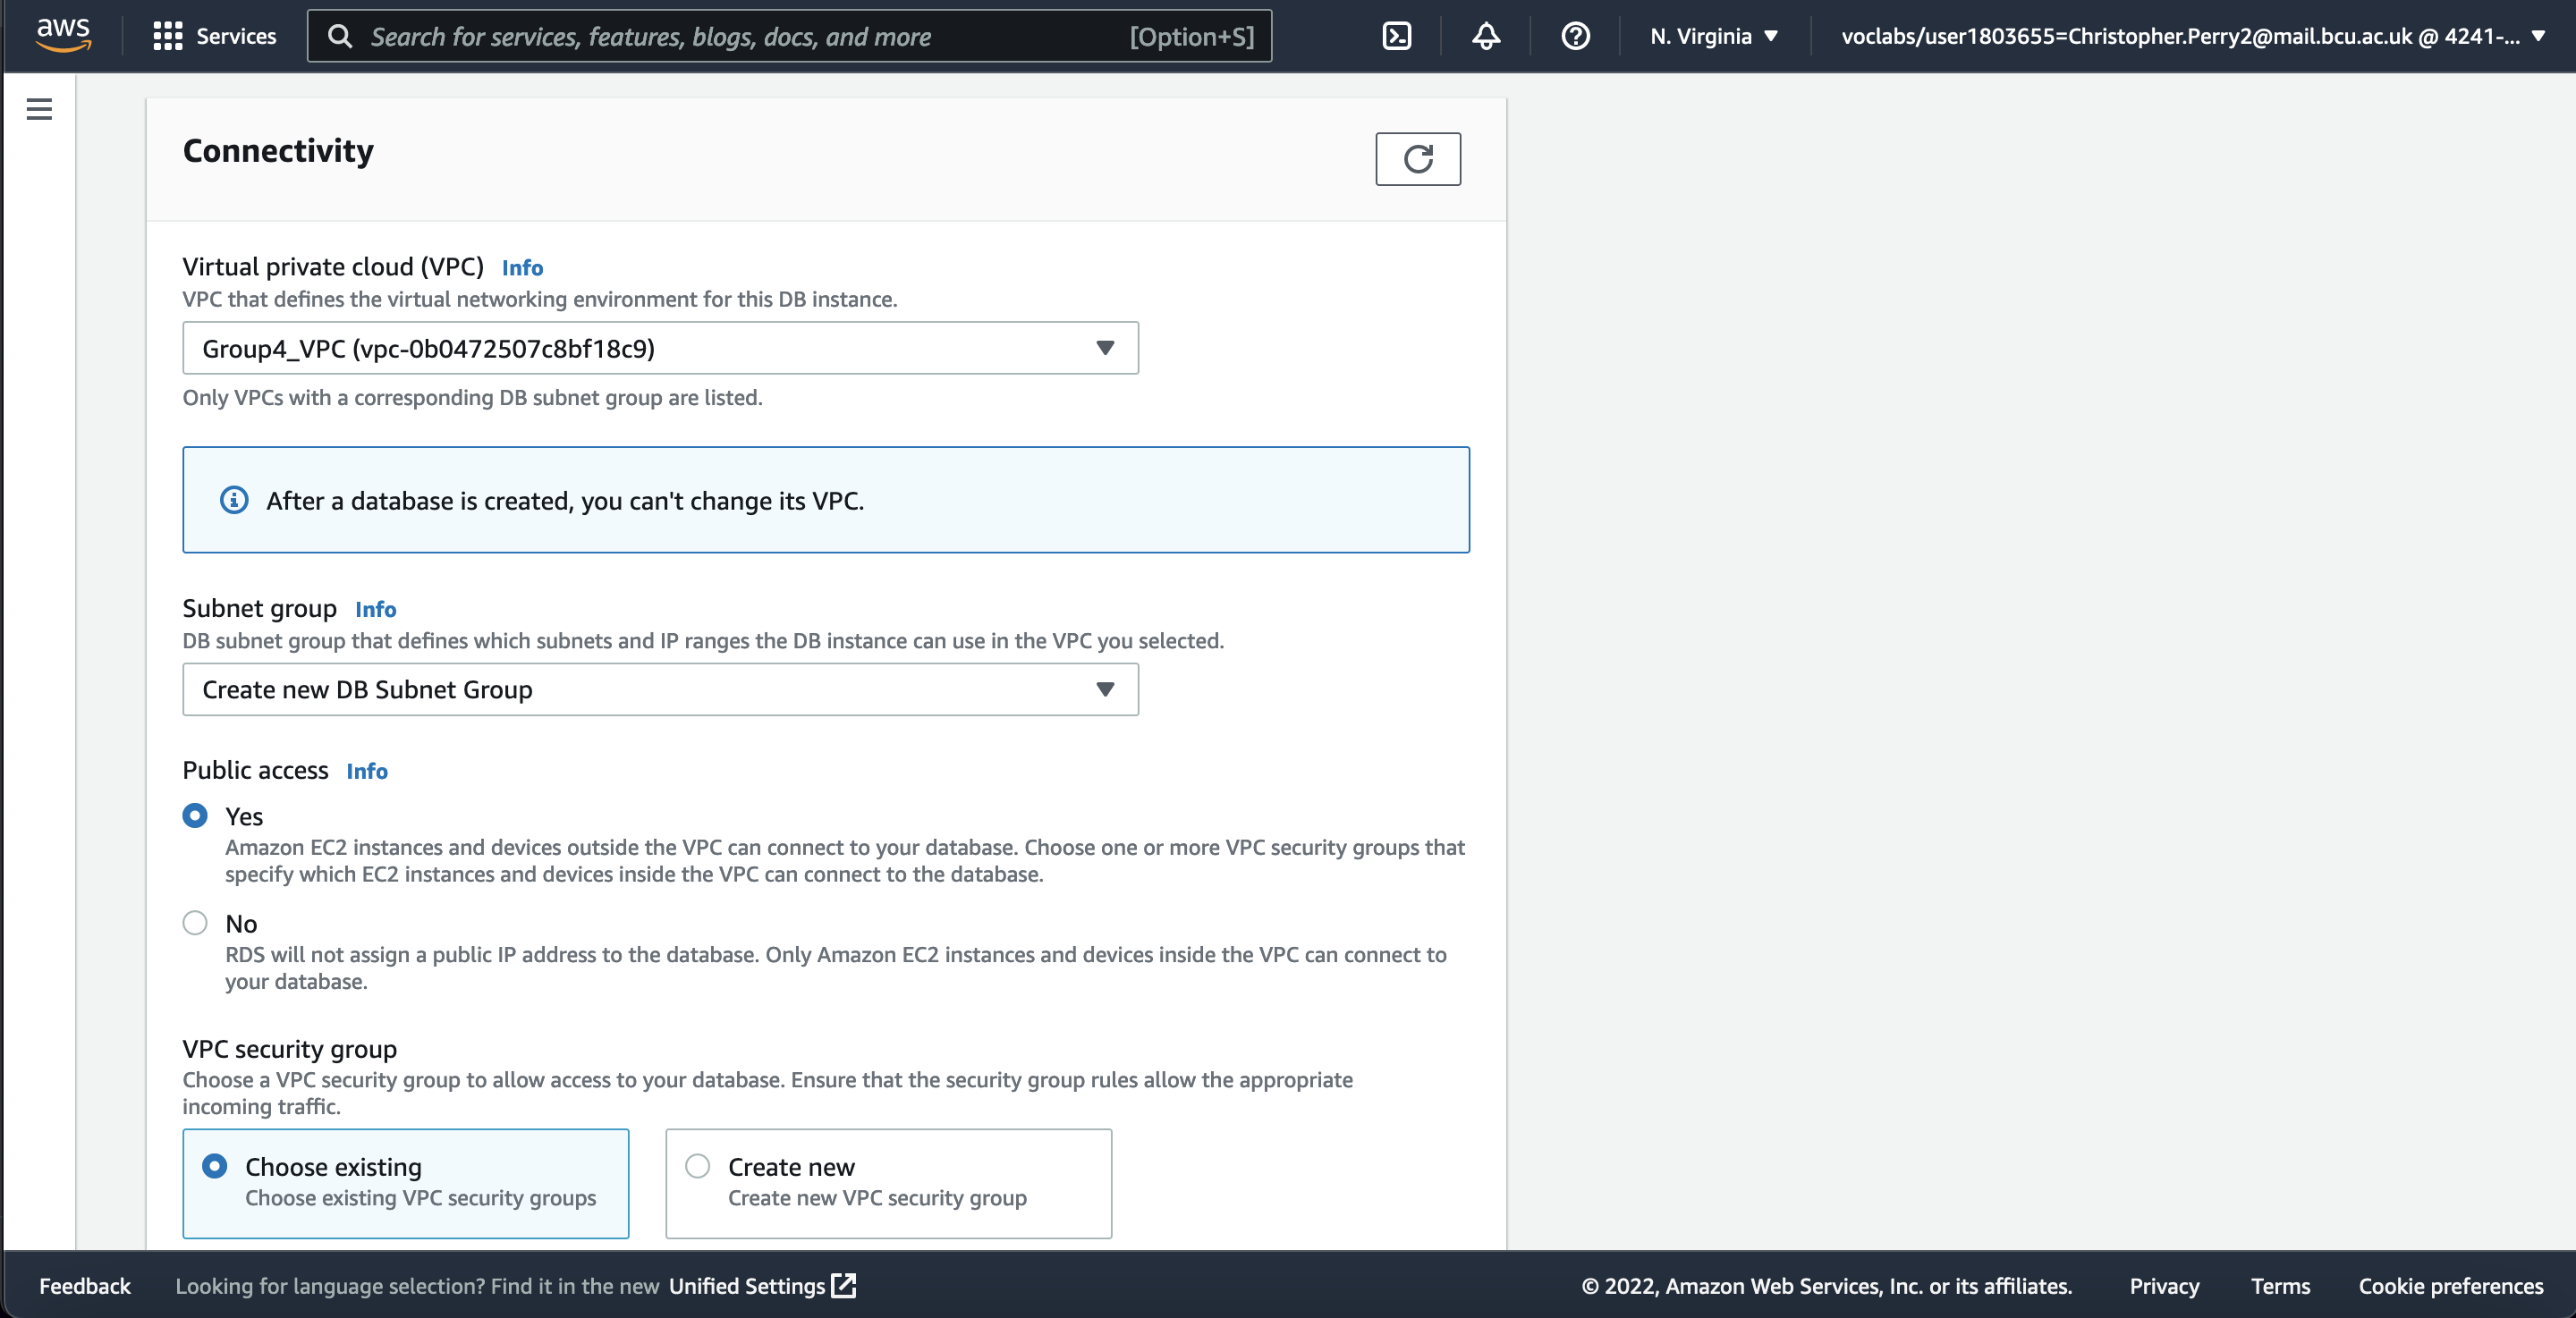
\includegraphics[width=\textwidth]{resources/rds/rds-connectivity-1}
    \caption{Selection of VPC and subnet groups.}
    \label{fig:rds-connecting}
\end{figure}

\clearpage
Several database engine options are compatible with RDS, including Amazon Aurora, MySQL, MariaDB, and more.
MySQL was chosen for this RDS instance as it is the same database engine used in the local deployment of
\textit{Digital-Ink} within \mintinline{zsh}|docker-compose|.

\begin{figure}[!htbp]
    \centering
    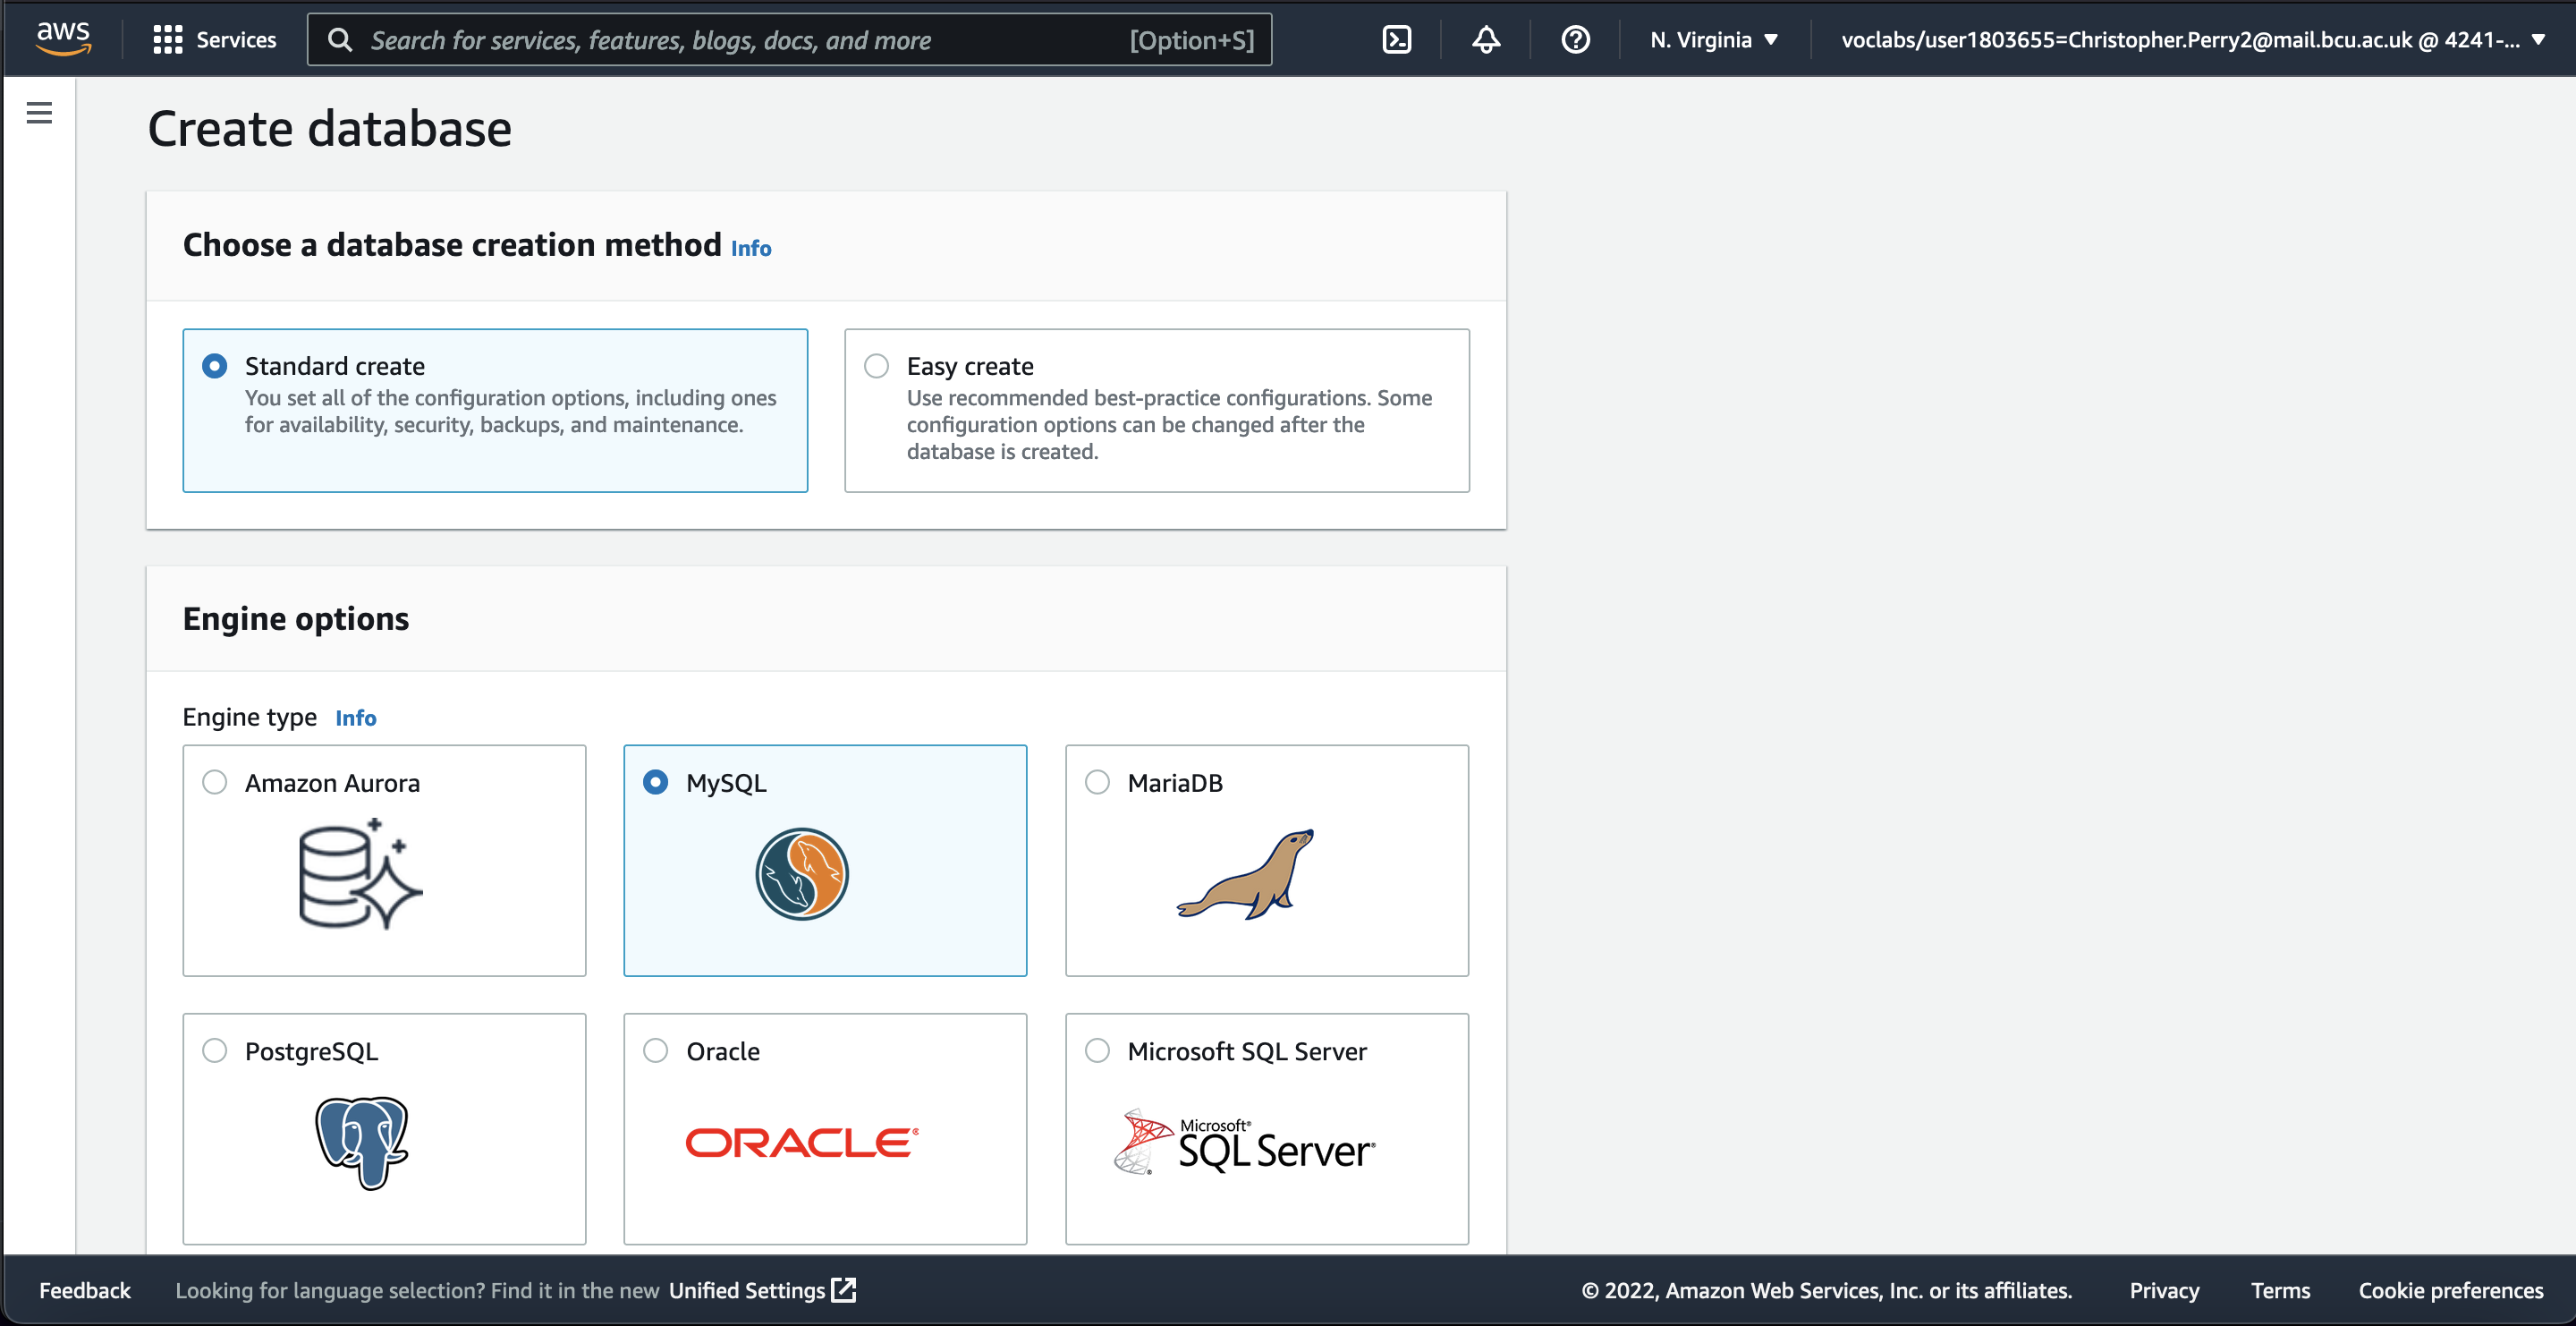
\includegraphics[width=\textwidth]{resources/rds/rds-create-engine}
    \caption{Selection of database engine.}
    \label{fig:rds-engine}
\end{figure}

The database template Dev/Test was selected as it was the cheapest tier that granted support for creating an RDS
instance with multiple availability zones.
The "free tier" provides no support for multiple-AZ deployment.

\begin{figure}[!htbp]
    \centering
    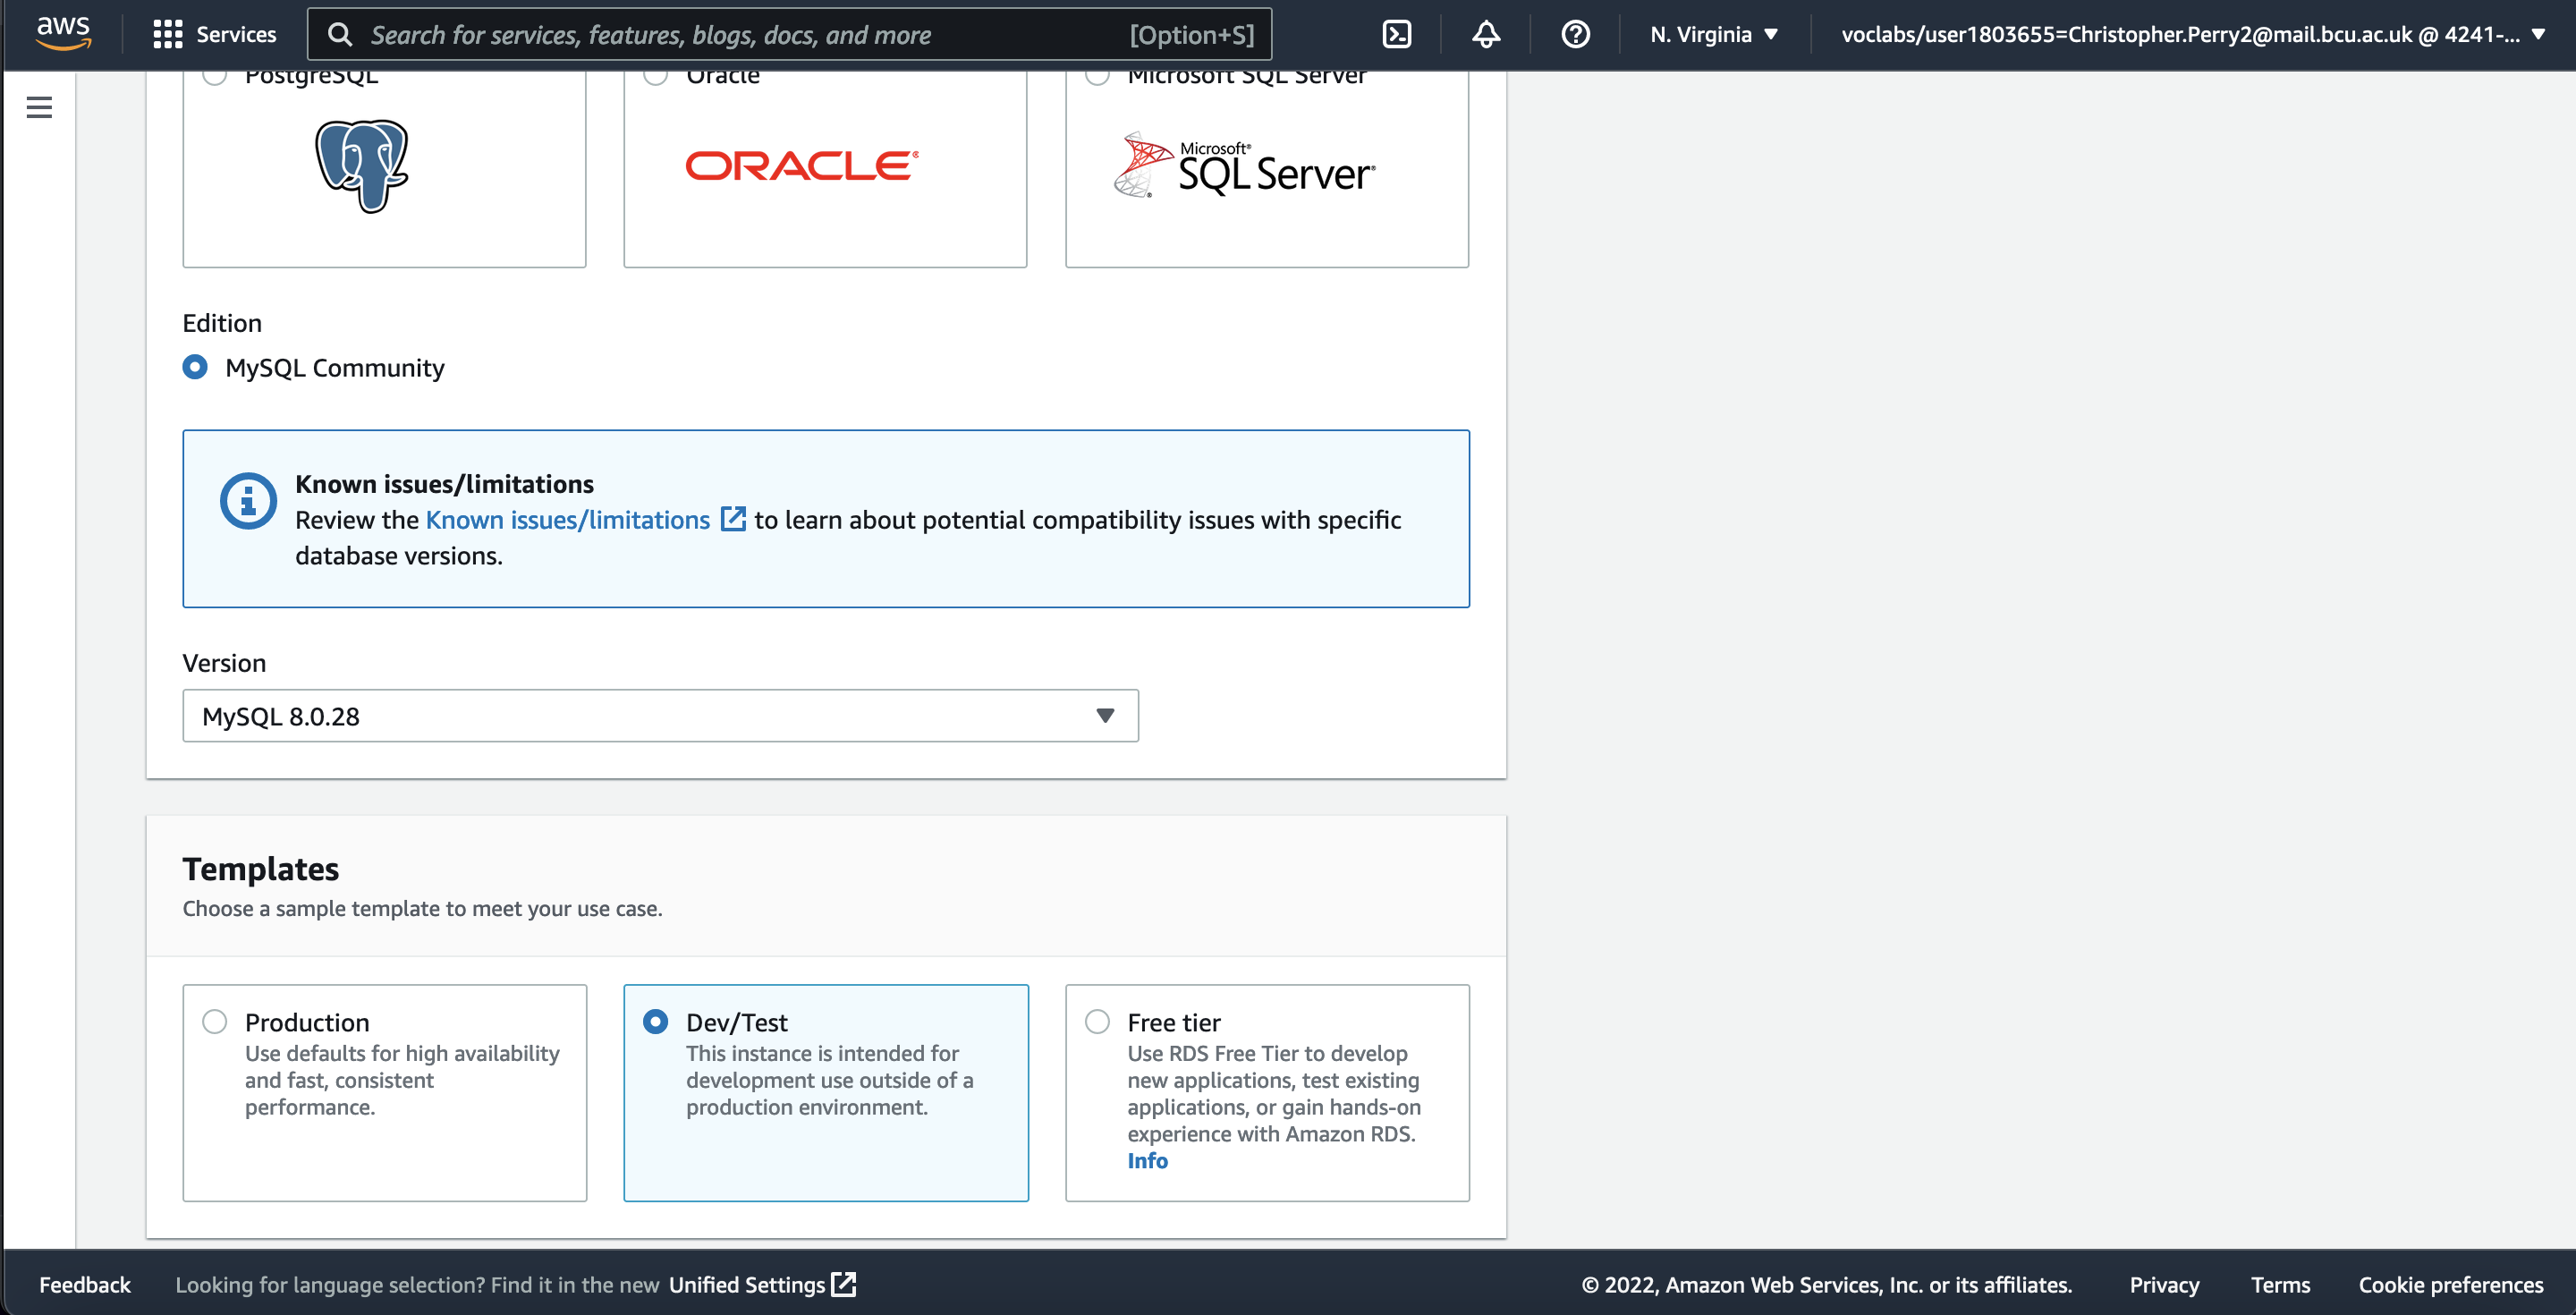
\includegraphics[width=\textwidth]{resources/rds/rds-templates}
    \caption{Selection of database template.}
    \label{fig:rds-templates}
\end{figure}

\clearpage
A micro-sized RDS instance was selected to reduce AWS billing costs where possible.
Figure~\ref{fig:rds-costs} details the estimated RDS cost per month.

\begin{figure}[!htbp]
    \centering
    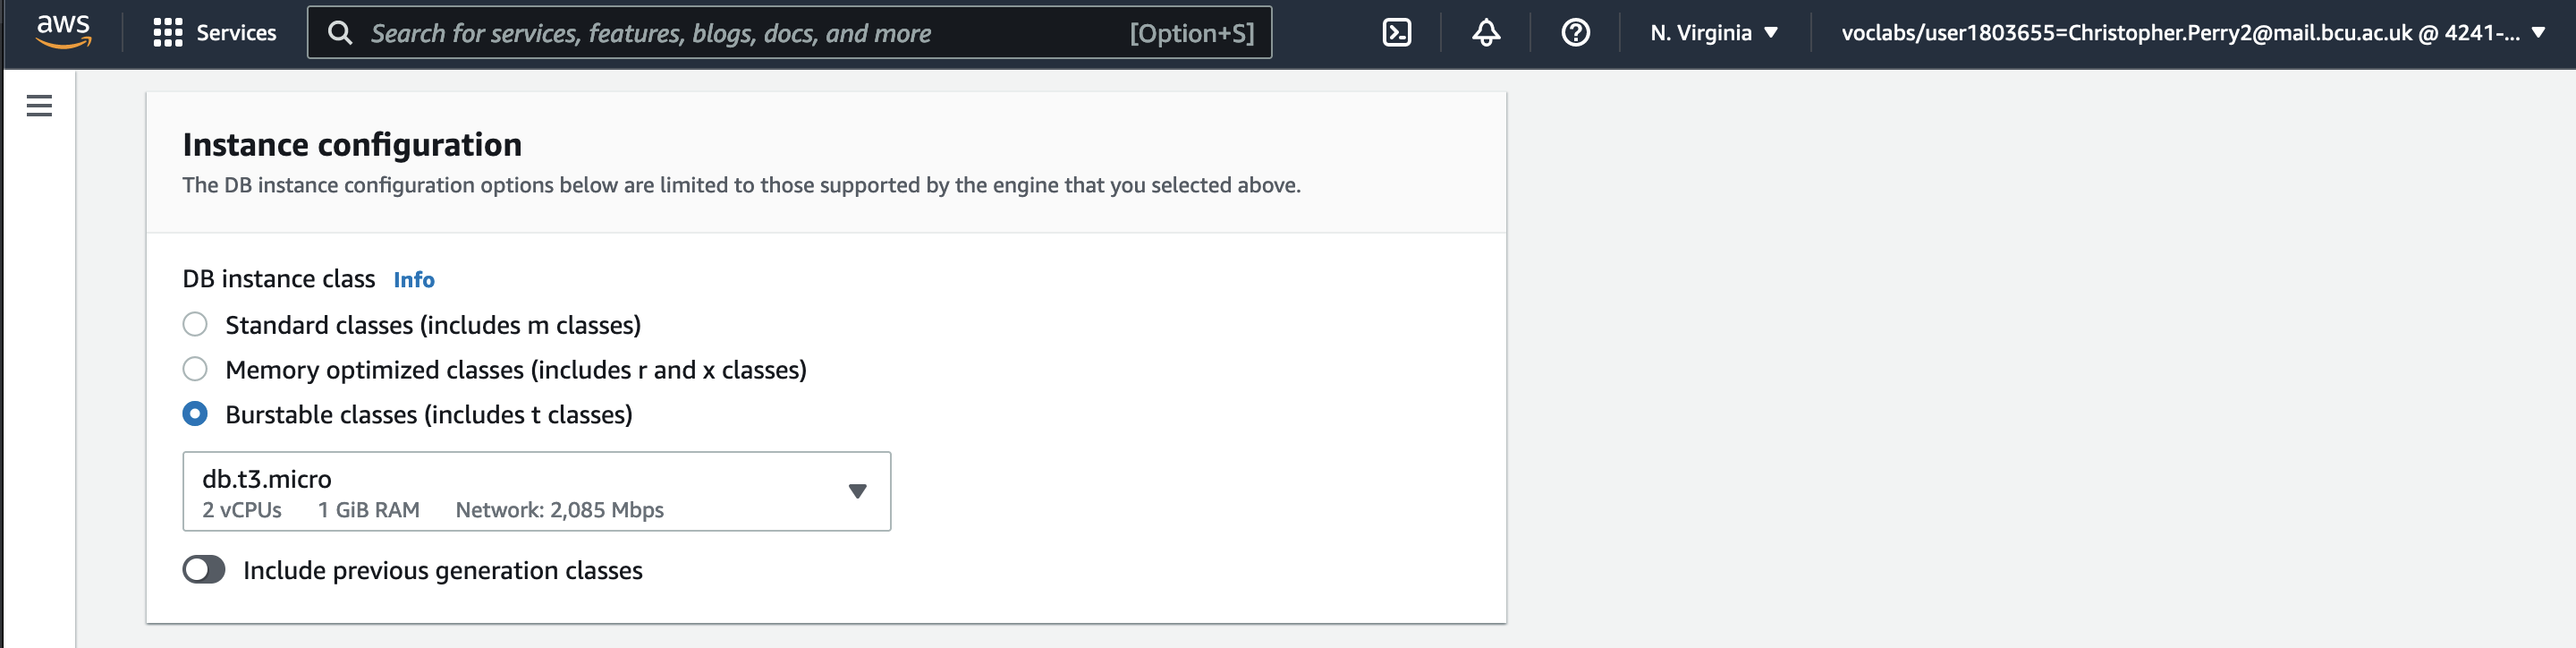
\includegraphics[width=125mm]{resources/rds/rds-instance-config}
    \caption{Selection of RDS Instance Size.}
    \label{fig:rds-instance-conf}
\end{figure}

\begin{figure}[!htbp]
    \centering
    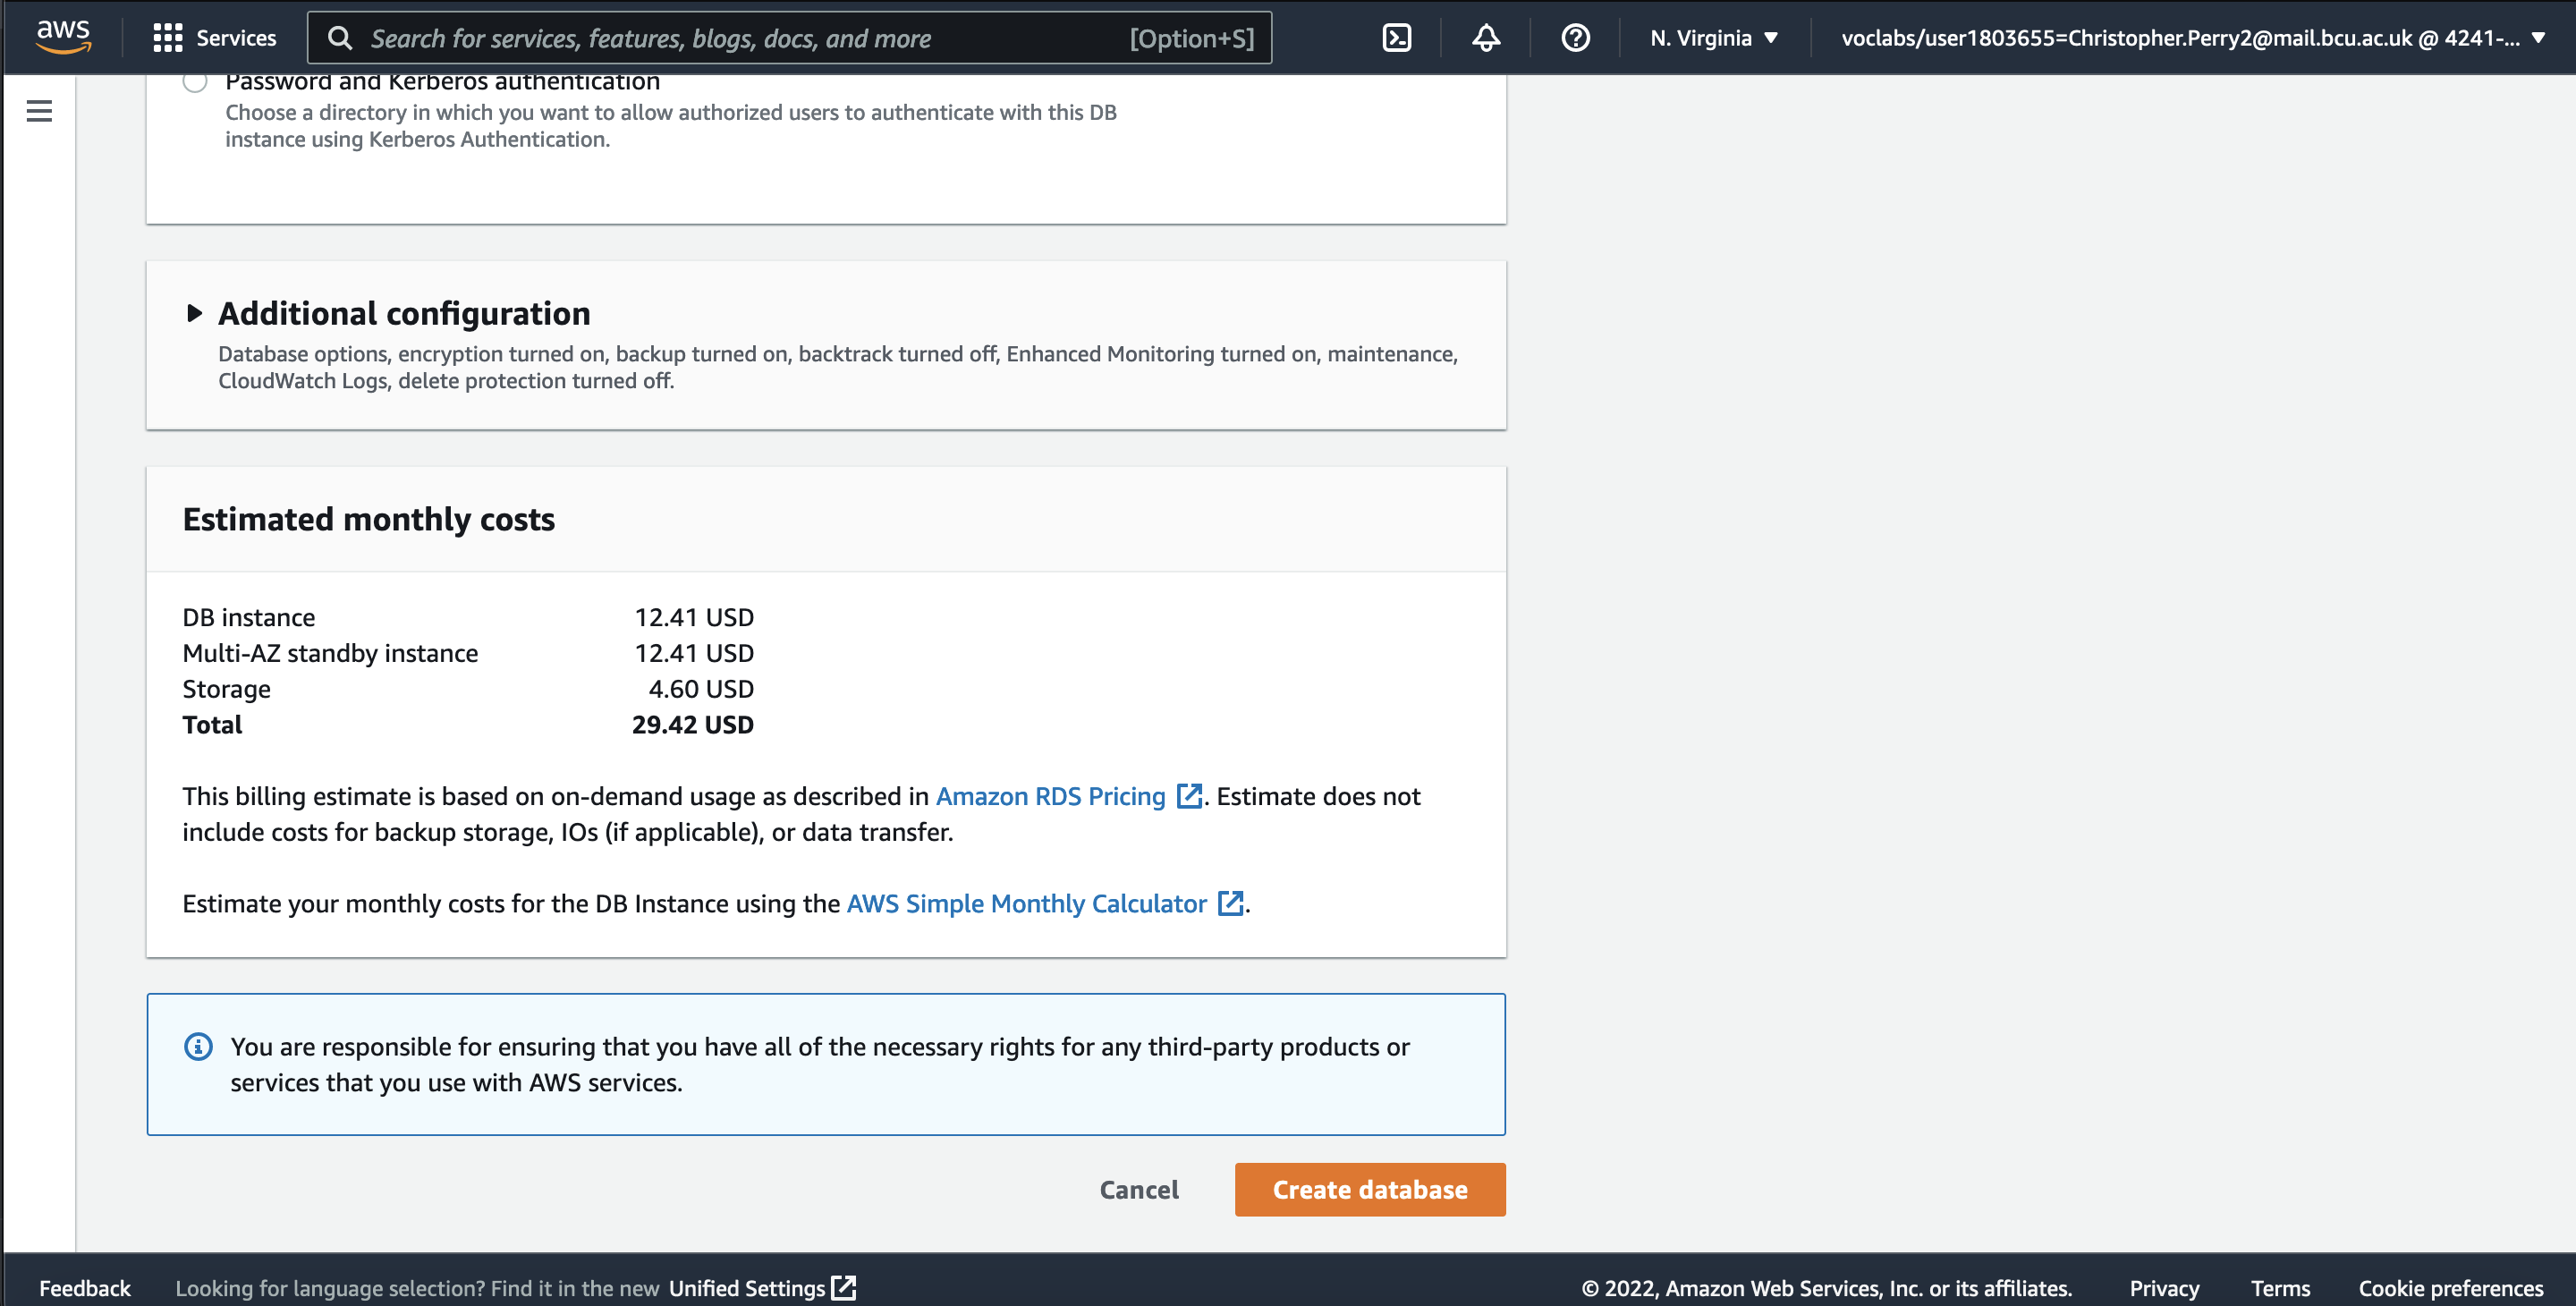
\includegraphics[width=125mm]{resources/rds/rds-monthly-costs}
    \caption{Estimated Monthly RDS Cost.}
    \label{fig:rds-costs}
\end{figure}

\clearpage
For additional security, a VPC security group is selected for the database.
The previously created security group is selected.
Additionally, RDS login details must be configured.
A master username of \mintinline{zsh}|admin| was chosen, and a password was automatically generated
by AWS with the current best security practices.

\begin{figure}[!htbp]
    \centering
    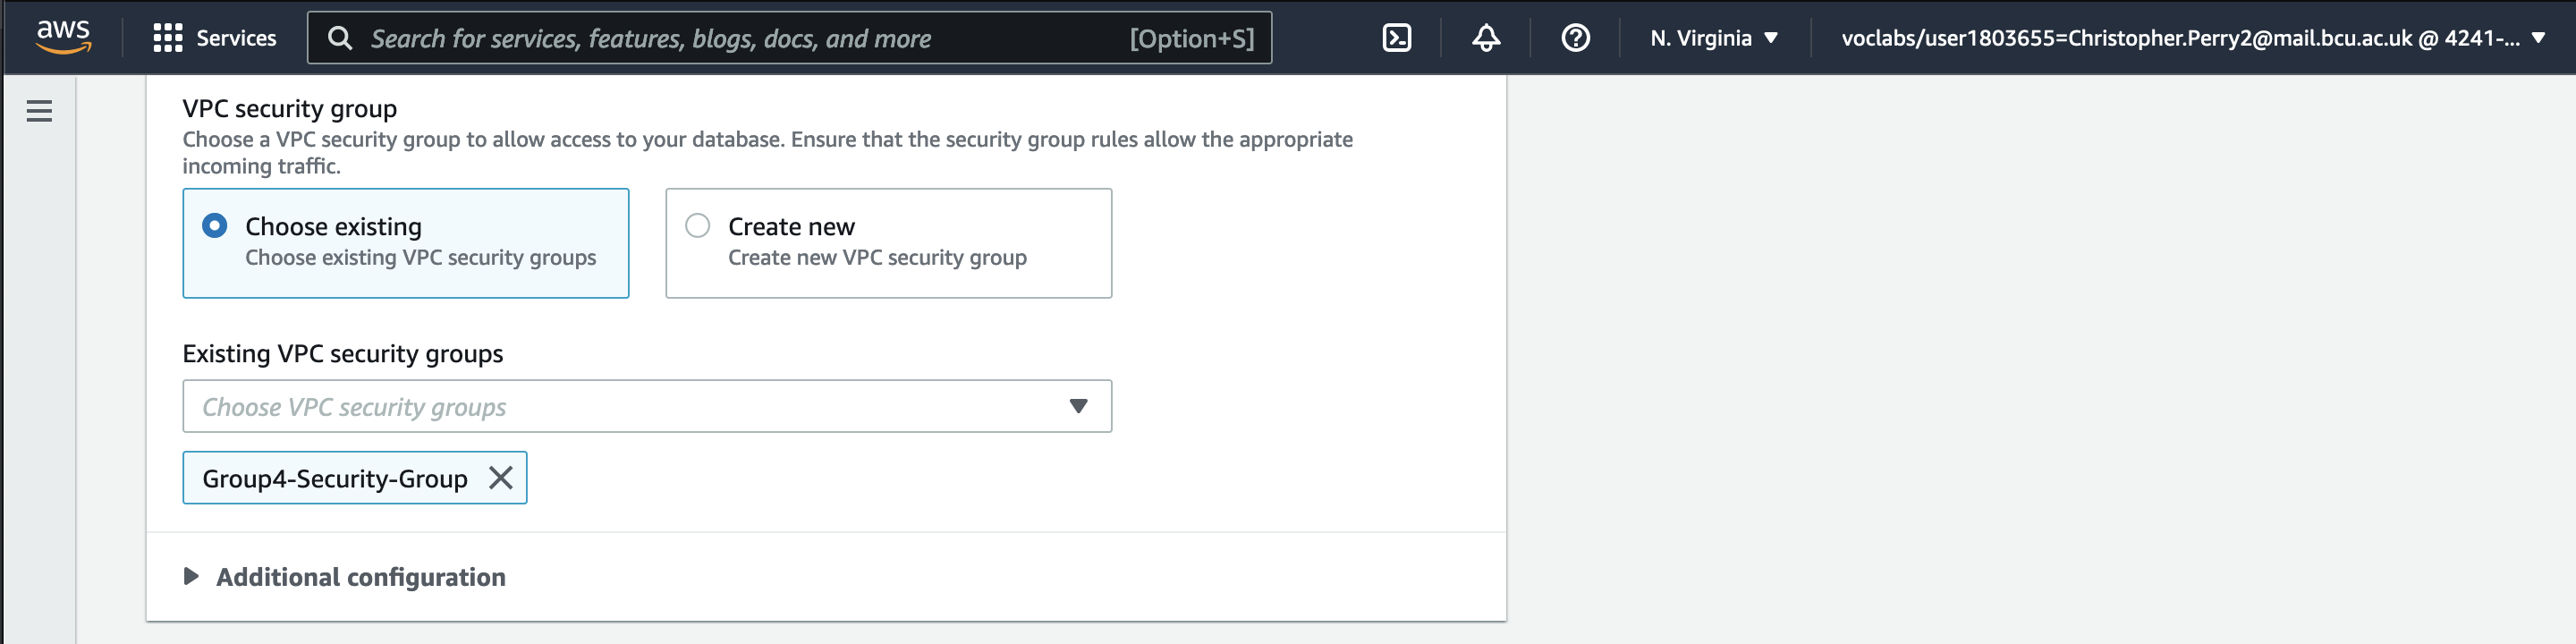
\includegraphics[width=\textwidth]{resources/rds/rds-security-group}
    \caption{Selection of RDS security group.}
    \label{fig:rds-security}
\end{figure}

\begin{figure}[!htbp]
    \centering
    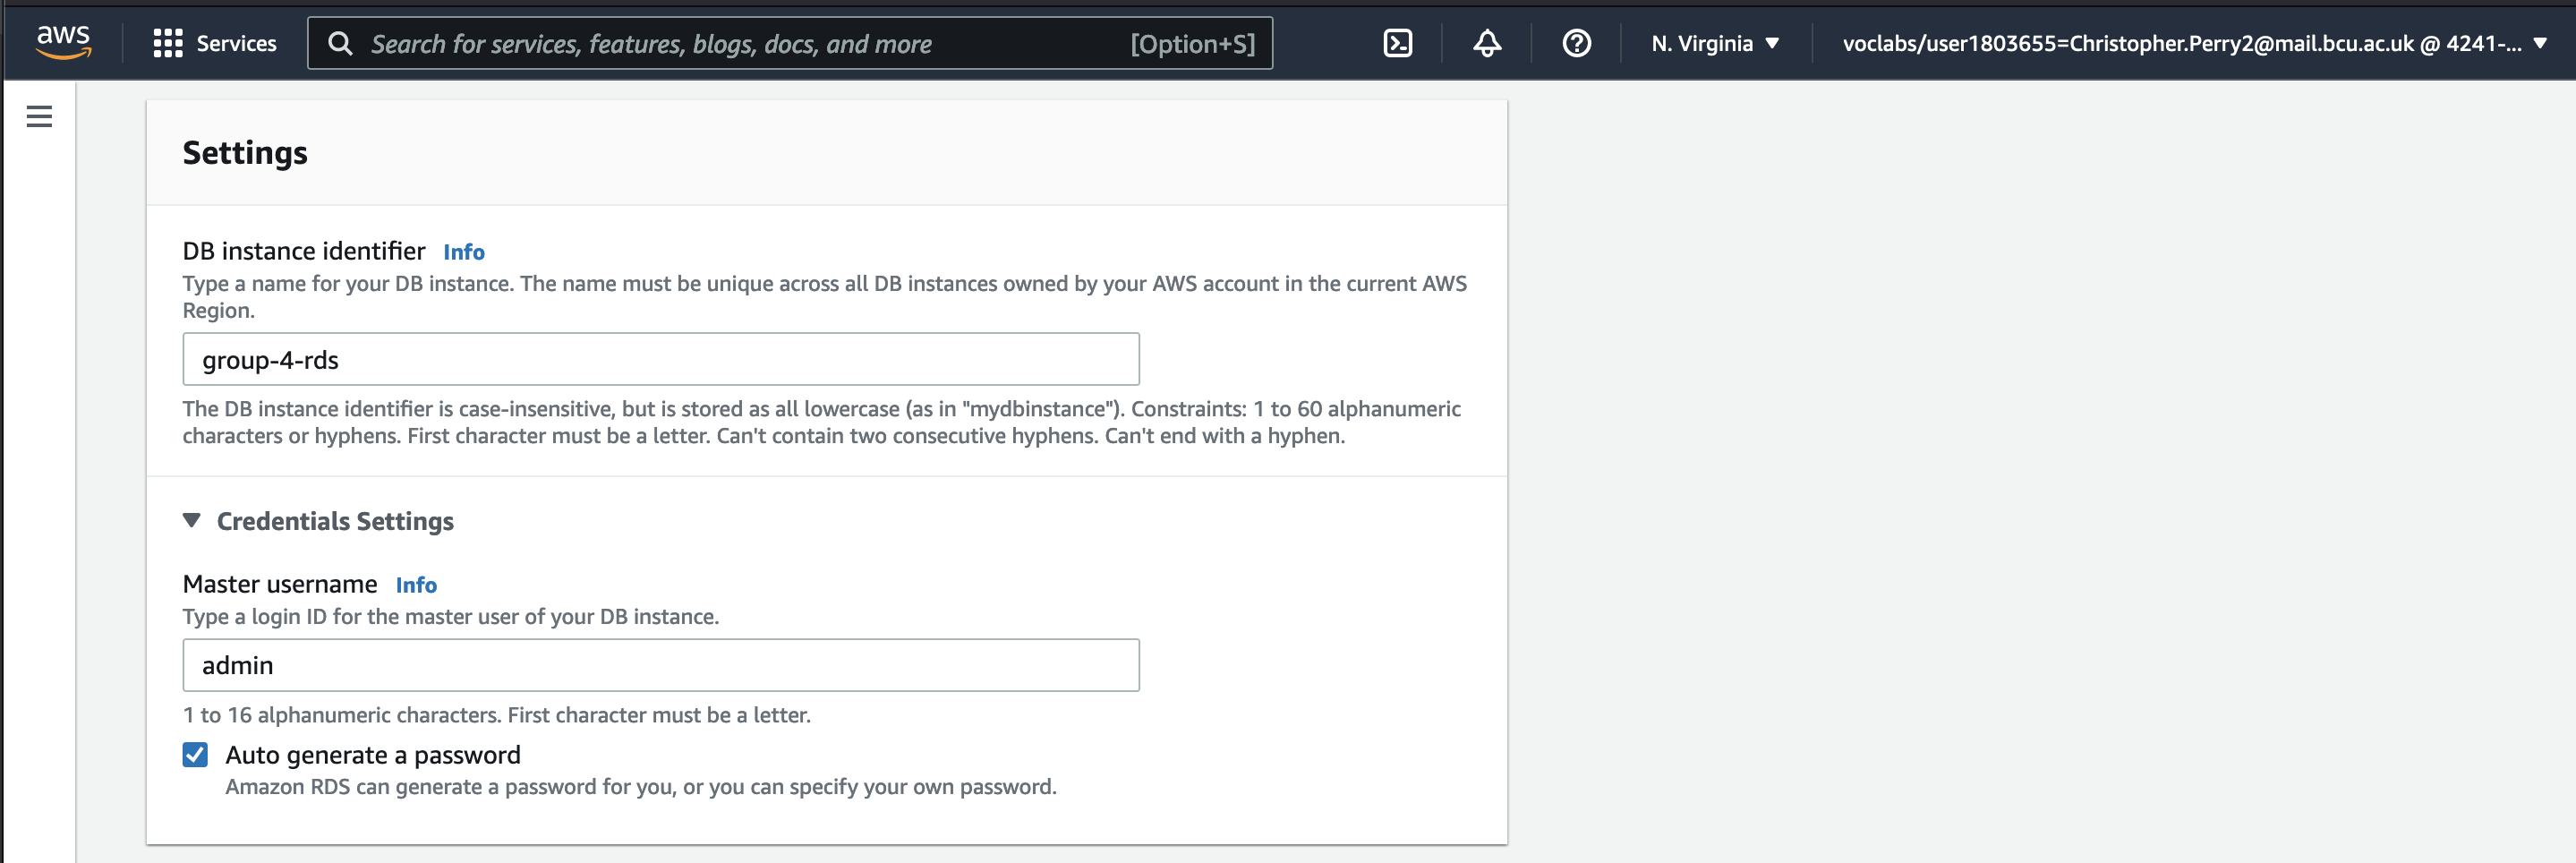
\includegraphics[width=\textwidth]{resources/rds/rds-settings}
    \caption{Generating credentials for RDS authentication.}
    \label{fig:rds-settings}
\end{figure}

\clearpage
A selection of how much storage the RDS instance is able to access should be made.
It was decided that, due to billing constraints, a small amount of storage, with size to automatically grow if
the application was presented with more users, was most appropriate.

\begin{figure}[!htbp]
    \centering
    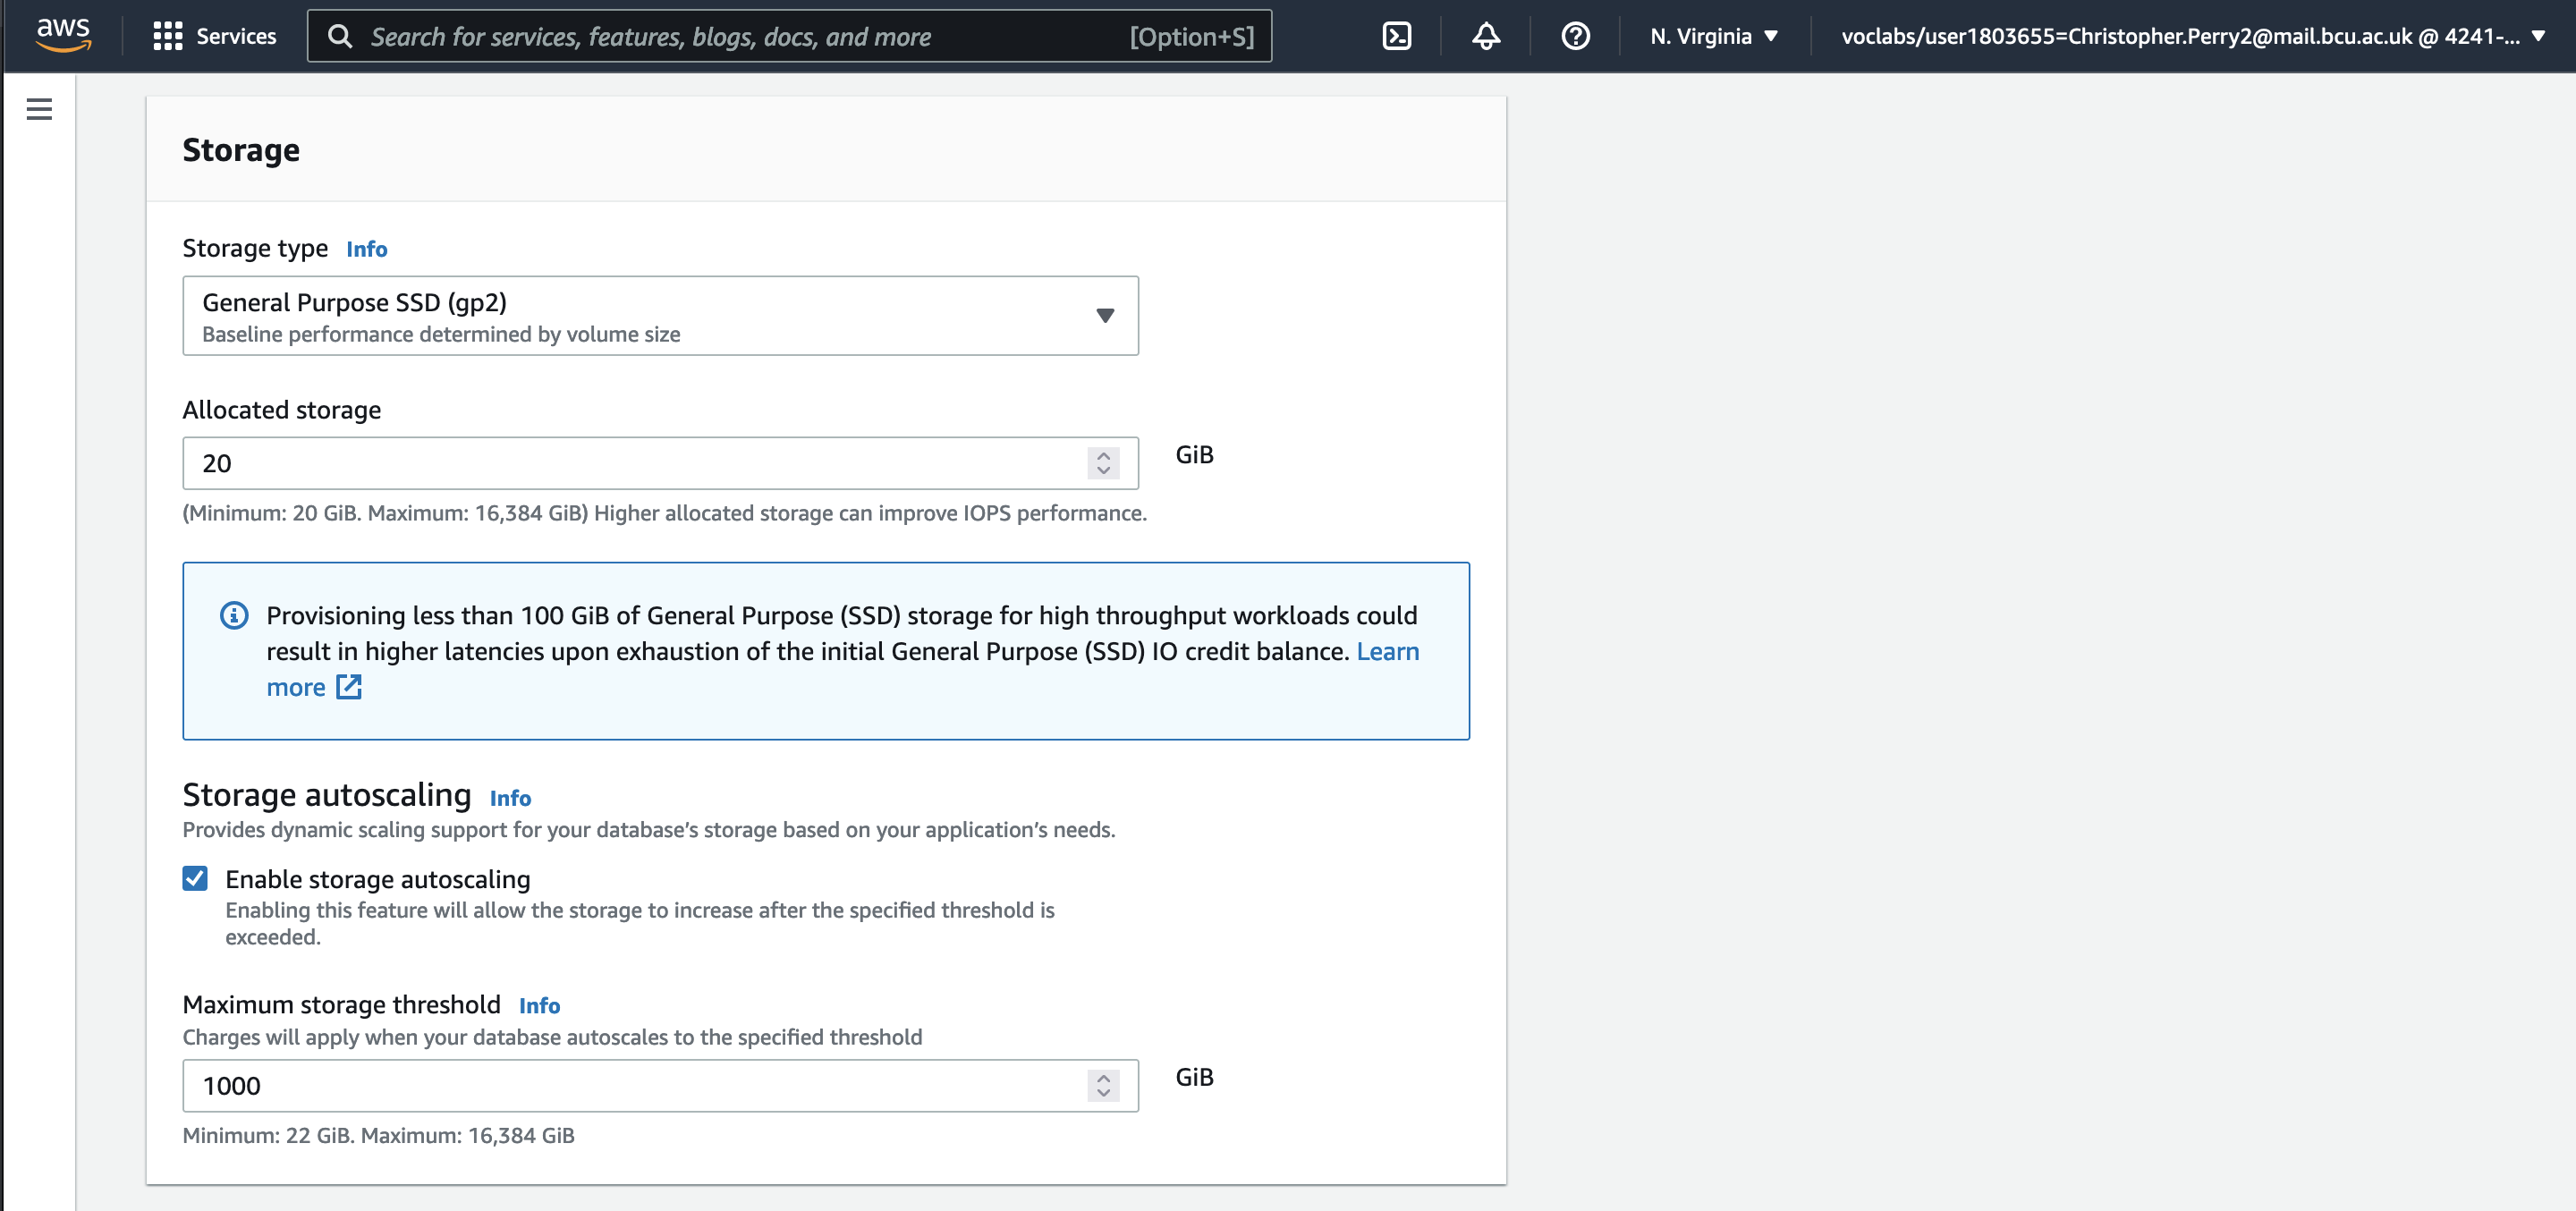
\includegraphics[width=125mm]{resources/rds/rds-storage}
    \caption{Selection of Storage Parameters.}
    \label{fig:rds-storage}
\end{figure}

MySQL was selected as it was the same database engine that the web application was originally using within Docker.
The tables were generated using the command \mintinline{zsh}|php artisan migrate|, which generated all of the necessary
tables by using the migration scripts.

\begin{figure}[!htbp]
    \centering
    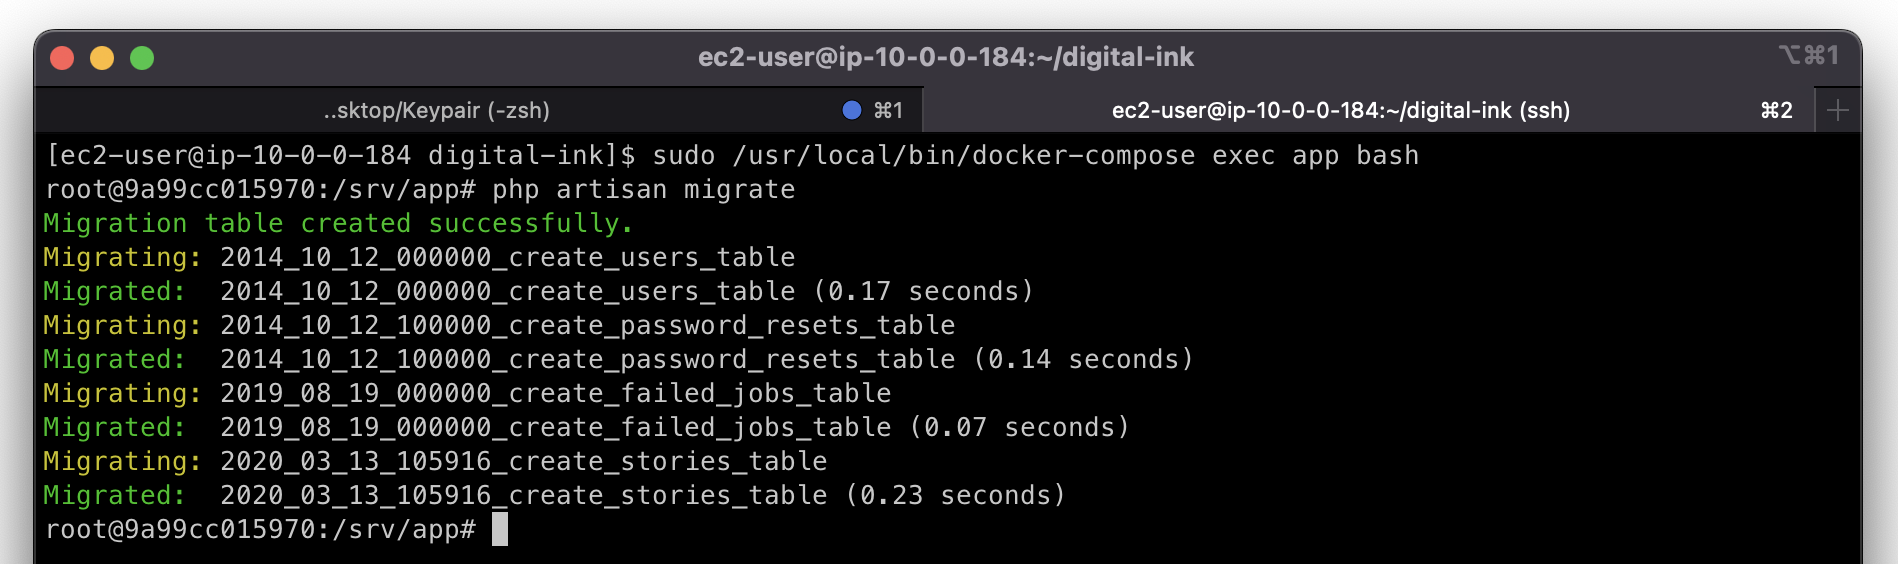
\includegraphics[width=\textwidth]{resources/rds/rds-tables-creation}
    \caption{Creation of RDS tables.}
    \label{fig:rds-tables}
\end{figure}

\clearpage
\section{Accessing the Database}\label{sec:accessing-the-new-database}
MySQL was installed on the EC2 instance in order to sign in to the new database and create tables.

\begin{figure}[!htbp]
    \centering
    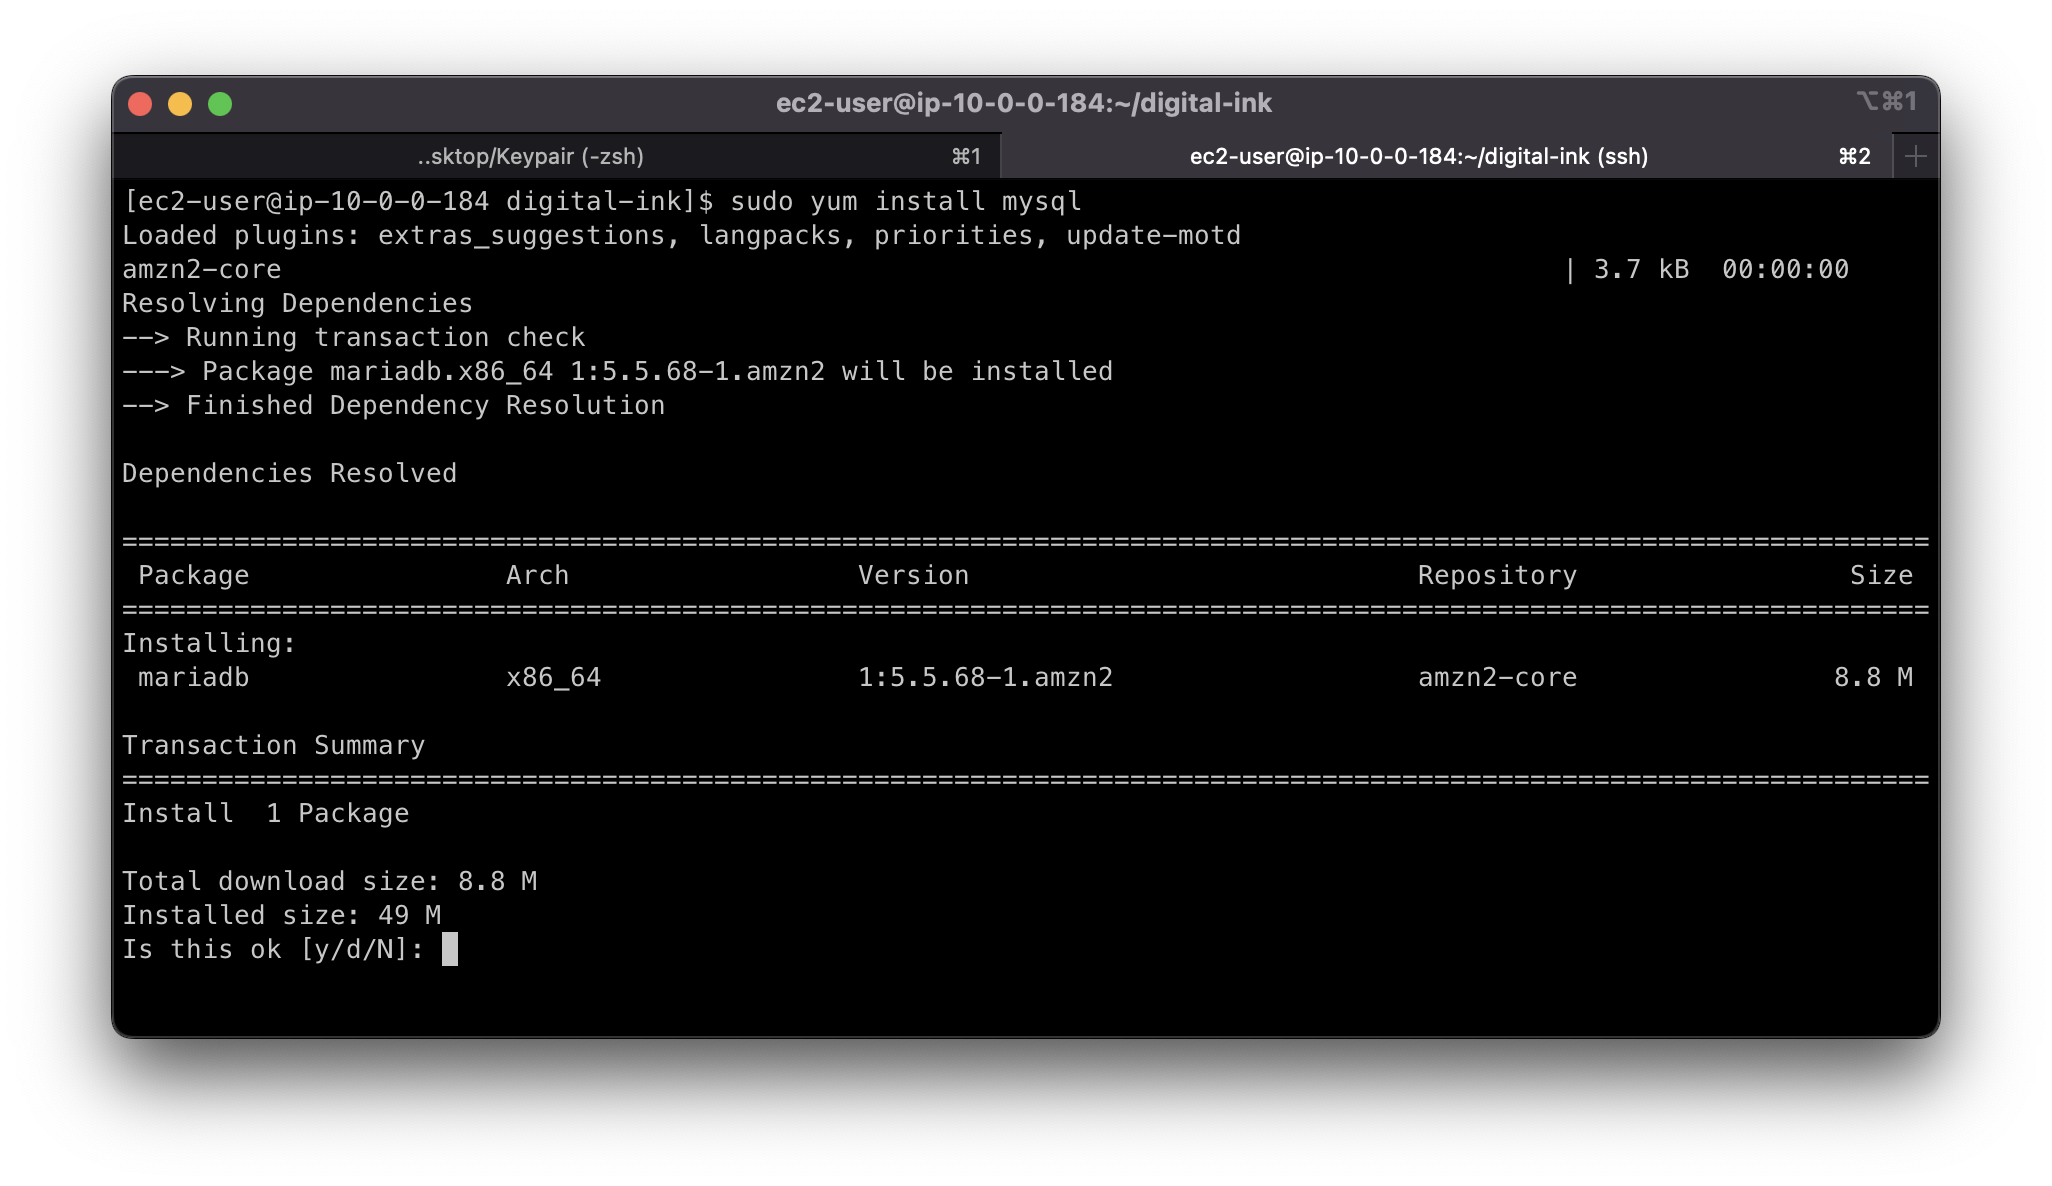
\includegraphics[width=125mm]{resources/rds/rds-mysql-install}
    \caption{Installation of MySQL on the EC2 instance.}
    \label{fig:rds-msql-install}
\end{figure}

MySQL was installed manually on the EC2 instance to provide access to the \mintinline{zsh}|mysql| command,
which allowed for signing into the database.
The command \mintinline{zsh}|mysql -h \$ENDPOINT -u admin -p\$PASSWORD| was then used.

\begin{figure}[!htbp]
    \centering
    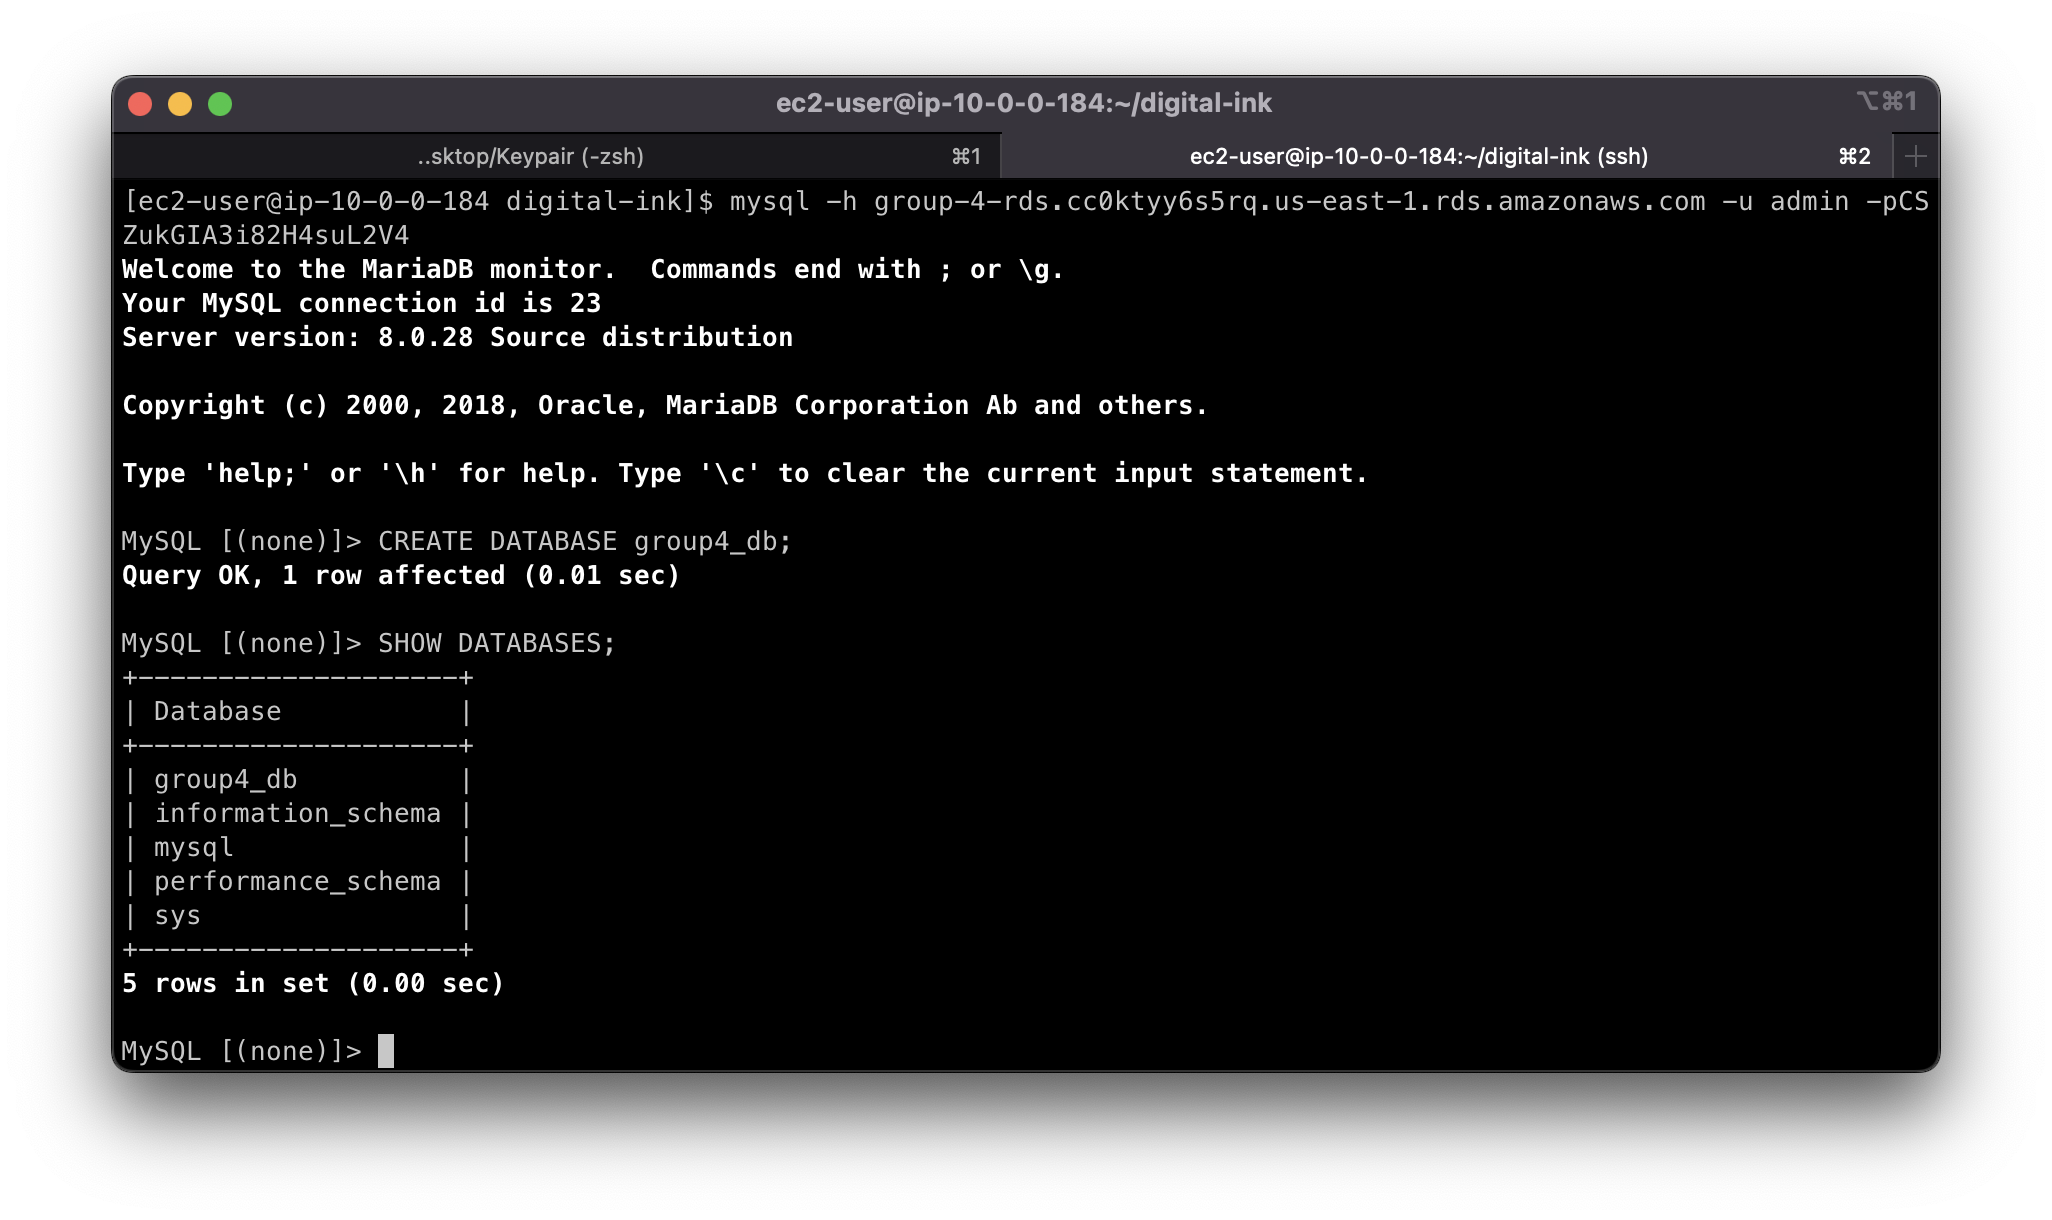
\includegraphics[width=125mm]{resources/rds/rds-database-creation}
    \caption{Creation of a database.}
    \label{fig:rds-db-create-2}
\end{figure}

\clearpage
The web application required a database table to be created manually before the database migrations could be run, so
following command was used within the RDS SQL environment: \mintinline{sql}|CREATE DATABASE group4_db;|.

\begin{figure}[!htbp]
    \centering
    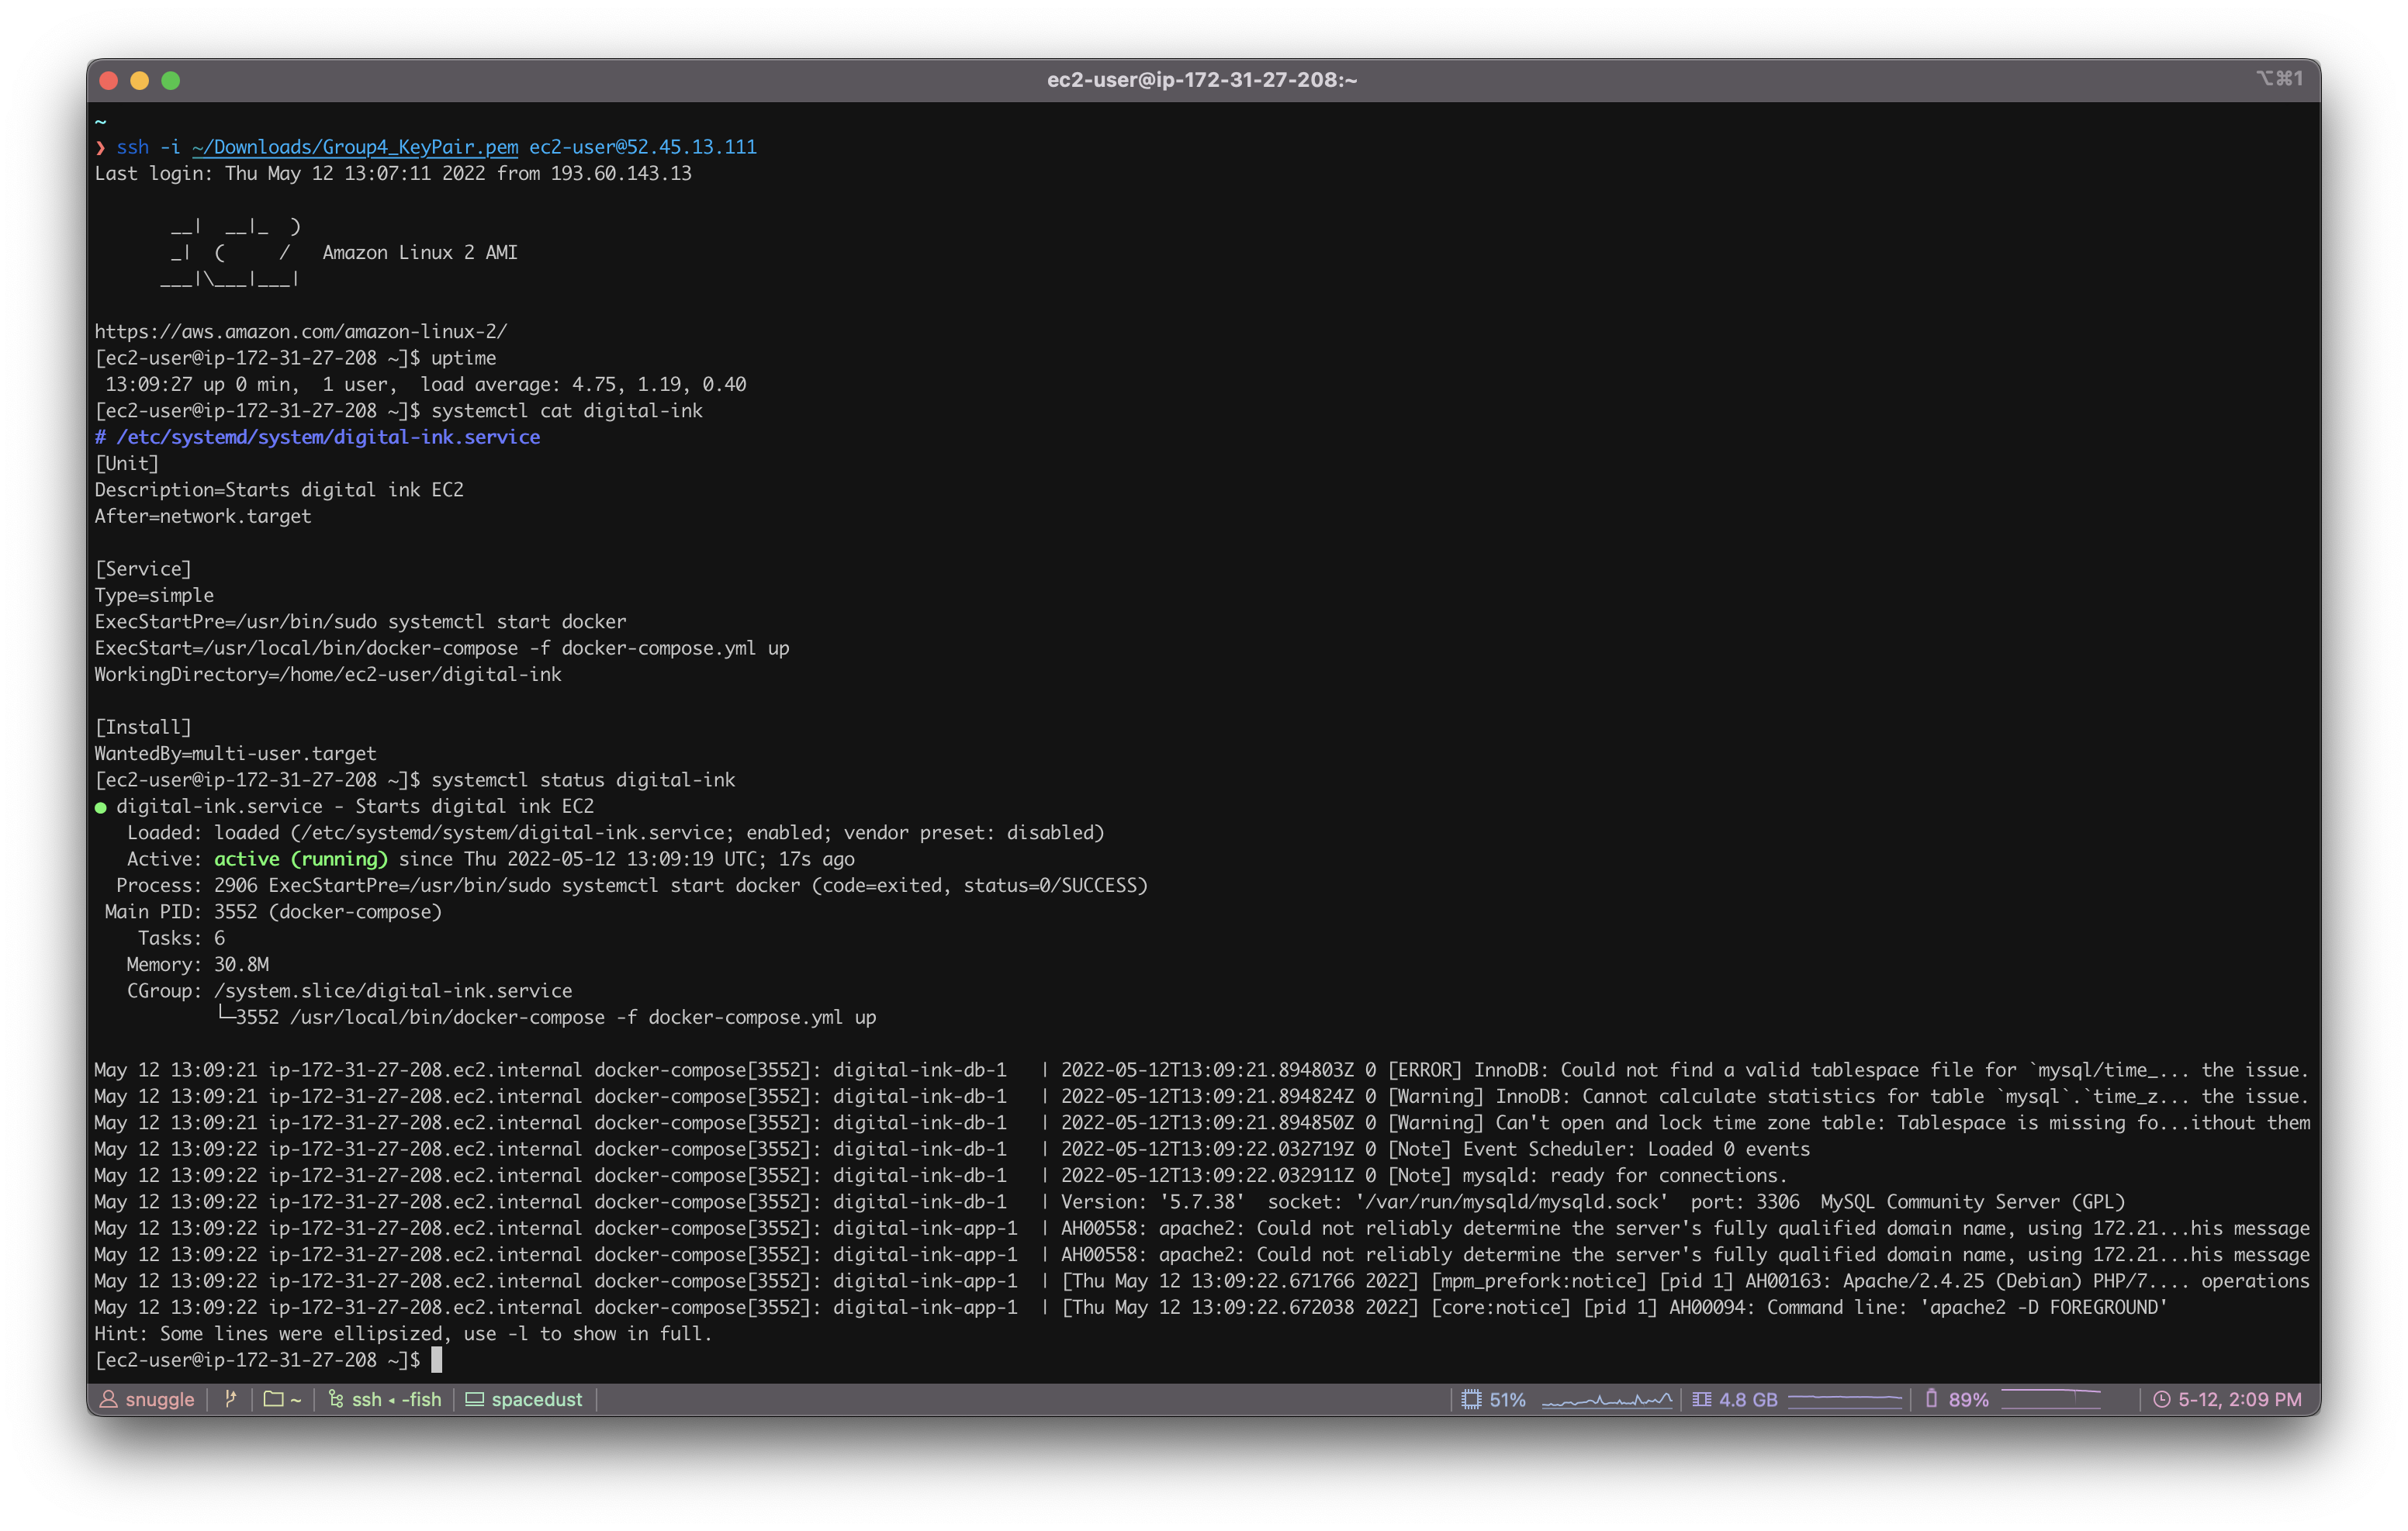
\includegraphics[width=125mm]{resources/rds/envupdate}
    \caption{Changing the database endpoint from Docker to AWS RDS.}
    \label{fig:rds-env-update}
\end{figure}

After the database was set up, tested and working, the old MySQL docker container was removed from the docker-compose
file.

\begin{figure}[!htbp]
    \centering
    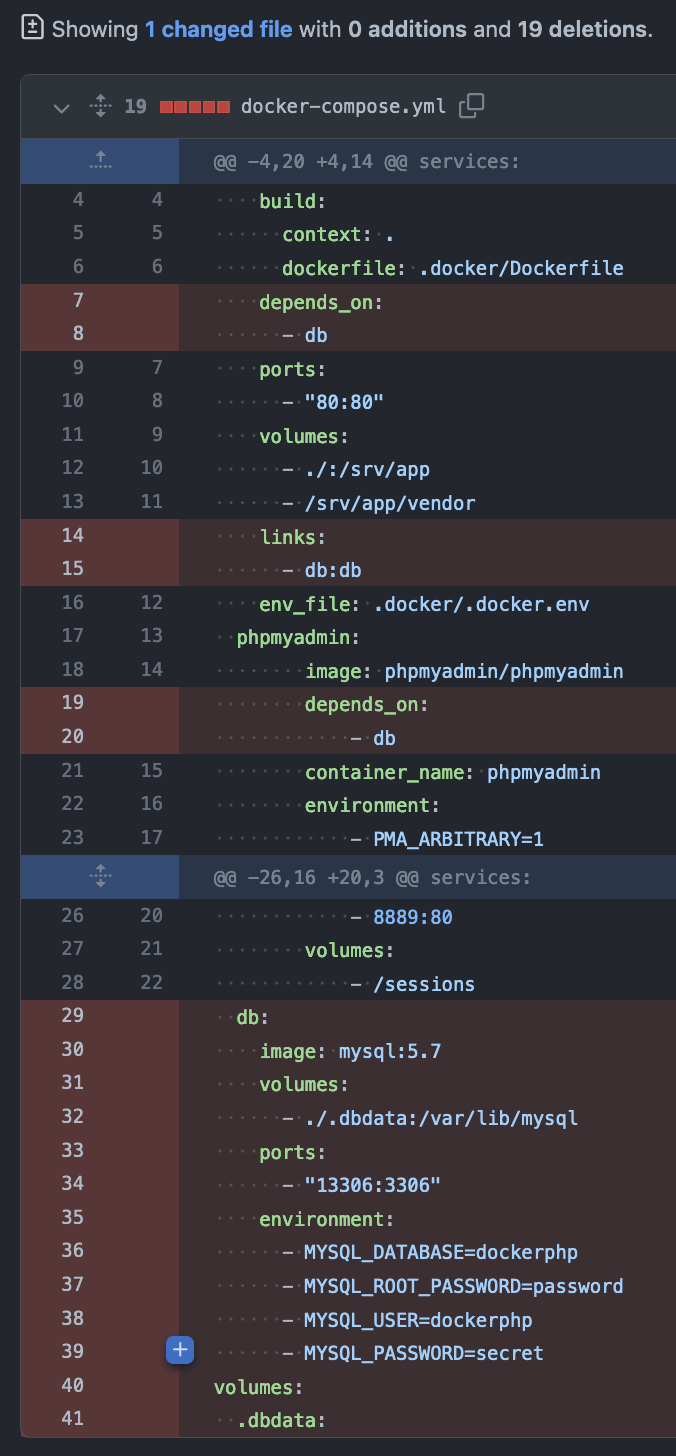
\includegraphics[width=50mm]{resources/rds/docker}
    \caption{Removal of database from docker file.}
    \label{fig:rds-rm-docker-compose}
\end{figure}

As old database was no longer needed within the \mintinline{zsh}|docker-compose.yml| file, the container was removed and
only Amazon RDS was used.
